% -*- Mode:TeX -*-

%% IMPORTANT: The official thesis specifications are available at:
%%            http://libraries.mit.edu/archives/thesis-specs/
%%
%%            Please verify your thesis' formatting and copyright
%%            assignment before submission.  If you notice any
%%            discrepancies between these templates and the 
%%            MIT Libraries' specs, please let us know
%%            by e-mailing thesis@mit.edu

%% The documentclass options along with the pagestyle can be used to generate
%% a technical report, a draft copy, or a regular thesis.  You may need to
%% re-specify the pagestyle after you \include  cover.tex.  For more
%% information, see the first few lines of mitthesis.cls. 

%\documentclass[12pt,vi,twoside]{mitthesis}
%%
%%  If you want your thesis copyright to you instead of MIT, use the
%%  ``vi'' option, as above.
%%
%\documentclass[12pt,twoside,leftblank]{mitthesis}
%%
%% If you want blank pages before new chapters to be labelled ``This
%% Page Intentionally Left Blank'', use the ``leftblank'' option, as
%% above. 

\documentclass[12pt,twoside]{mitthesis}
\usepackage{lgrind}
%% These have been added at the request of the MIT Libraries, because
%% some PDF conversions mess up the ligatures.  -LB, 1/22/2014
\usepackage{cmap}
\usepackage[T1]{fontenc}
\pagestyle{plain}
\usepackage{verbatim}
\usepackage{array}
\usepackage{float}
\usepackage{amsmath}
\usepackage{amssymb}
\usepackage{graphicx}
\usepackage{enumitem}
\usepackage{tikz}
\usetikzlibrary{shapes,arrows,positioning,calc}
%\usepackage{hyperref}
%\hypersetup{colorlinks=true, allcolors=[rgb]{0.3,0.3,0.8}}

\graphicspath{{../fig/}}

\tikzstyle{block} = [draw, rectangle, rounded corners=0.1cm,
    minimum height=3em, minimum width=6em, text=black, align=center]
\tikzstyle{sum} = [draw, circle, fill=white, node distance=1.5cm, minimum size=1cm, text=black]
\tikzstyle{gain} = [draw, circle, color=olive!100, thick, fill=olive!5, node distance=1.5cm, minimum size=1cm, text=black]
\tikzstyle{input} = [coordinate]
\tikzstyle{output} = [coordinate]
\tikzstyle{pinstyle} = [pin edge={to-,thin,black}]
\tikzstyle{tri_gain} = [draw, isosceles triangle,
      		  fill=white, shape border rotate=180]
\tikzstyle{stage} = [draw, rectangle, rounded corners=0.1cm, align=center, minimum height=3em, minimum width=9em, color=gray!80, fill=blue!50!green!20, text = black, node distance=8cm, font=\bf]
\tikzstyle{row} = [draw, rectangle, rounded corners=0.1cm, align=center, minimum height=3em, minimum width=40em, text=black, color=gray!80, fill=gray!10]
\tikzstyle{note} = [align=center, minimum height=3.5em, minimum width=36em, text=black]
\tikzstyle{arr} = [draw, line width=0.8mm, ->, color=gray]


\begin{document}

% -*-latex-*-
% 
% For questions, comments, concerns or complaints:
% thesis@mit.edu
% 
%
% $Log: cover.tex,v $
% Revision 1.8  2008/05/13 15:02:15  jdreed
% Degree month is June, not May.  Added note about prevdegrees.
% Arthur Smith's title updated
%
% Revision 1.7  2001/02/08 18:53:16  boojum
% changed some \newpages to \cleardoublepages
%
% Revision 1.6  1999/10/21 14:49:31  boojum
% changed comment referring to documentstyle
%
% Revision 1.5  1999/10/21 14:39:04  boojum
% *** empty log message ***
%
% Revision 1.4  1997/04/18  17:54:10  othomas
% added page numbers on abstract and cover, and made 1 abstract
% page the default rather than 2.  (anne hunter tells me this
% is the new institute standard.)
%
% Revision 1.4  1997/04/18  17:54:10  othomas
% added page numbers on abstract and cover, and made 1 abstract
% page the default rather than 2.  (anne hunter tells me this
% is the new institute standard.)
%
% Revision 1.3  93/05/17  17:06:29  starflt
% Added acknowledgements section (suggested by tompalka)
% 
% Revision 1.2  92/04/22  13:13:13  epeisach
% Fixes for 1991 course 6 requirements
% Phrase "and to grant others the right to do so" has been added to 
% permission clause
% Second copy of abstract is not counted as separate pages so numbering works
% out
% 
% Revision 1.1  92/04/22  13:08:20  epeisach

% NOTE:
% These templates make an effort to conform to the MIT Thesis specifications,
% however the specifications can change.  We recommend that you verify the
% layout of your title page with your thesis advisor and/or the MIT 
% Libraries before printing your final copy.
\title{Shared Decision-Making and Control Between Humans and Adaptive Control Algorithms}

\author{Benjamin T. Thomsen}
% If you wish to list your previous degrees on the cover page, use the 
% previous degrees command:
%       \prevdegrees{A.A., Harvard University (1985)}
% You can use the \\ command to list multiple previous degrees
       \prevdegrees{B.Eng., McGill University (2015)}
\department{Department of Mechanical Engineering}

% If the thesis is for two degrees simultaneously, list them both
% separated by \and like this:
% \degree{Doctor of Philosophy \and Master of Science}
\degree{Master of Science}

% As of the 2007-08 academic year, valid degree months are September, 
% February, or June.  The default is June.
\degreemonth{June}
\degreeyear{2018}
\thesisdate{May 11, 2018}

%% By default, the thesis will be copyrighted to MIT.  If you need to copyright
%% the thesis to yourself, just specify the `vi' documentclass option.  If for
%% some reason you want to exactly specify the copyright notice text, you can
%% use the \copyrightnoticetext command.  
%\copyrightnoticetext{\copyright IBM, 1990.  Do not open till Xmas.}

% If there is more than one supervisor, use the \supervisor command
% once for each.
\supervisor{Anuradha M. Annaswamy}{Senior Research Scientist}

% This is the department committee chairman, not the thesis committee
% chairman.  You should replace this with your Department's Committee
% Chairman.
\chairman{Rohan Abeyaratne}{Chairman, Department Committee on Graduate Theses}

% Make the titlepage based on the above information.  If you need
% something special and can't use the standard form, you can specify
% the exact text of the titlepage yourself.  Put it in a titlepage
% environment and leave blank lines where you want vertical space.
% The spaces will be adjusted to fill the entire page.  The dotted
% lines for the signatures are made with the \signature command.
\maketitle

% The abstractpage environment sets up everything on the page except
% the text itself.  The title and other header material are put at the
% top of the page, and the supervisors are listed at the bottom.  A
% new page is begun both before and after.  Of course, an abstract may
% be more than one page itself.  If you need more control over the
% format of the page, you can use the abstract environment, which puts
% the word "Abstract" at the beginning and single spaces its text.

%% You can either \input (*not* \include) your abstract file, or you can put
%% the text of the abstract directly between the \begin{abstractpage} and
%% \end{abstractpage} commands.

% First copy: start a new page, and save the page number.
\cleardoublepage
% Uncomment the next line if you do NOT want a page number on your
% abstract and acknowledgments pages.
% \pagestyle{empty}
\setcounter{savepage}{\thepage}
\begin{abstractpage}
% $Log: abstract.tex,v $
% Revision 1.1  93/05/14  14:56:25  starflt
% Initial revision
% 
% Revision 1.1  90/05/04  10:41:01  lwvanels
% Initial revision
% 
%
%% The text of your abstract and nothing else (other than comments) goes here.
%% It will be single-spaced and the rest of the text that is supposed to go on
%% the abstract page will be generated by the abstractpage environment.  This
%% file should be \input (not \include 'd) from cover.tex.

This thesis addresses the problem of controlling a dynamical system subject to both parametric uncertainties and abrupt changes in the dynamic structure of the system, by proposing a shared control architecture predicated on a suitable division of responsibilities between supervisory human operators and adaptive control algorithms. Dynamical anomalies, such as the sudden introduction of unmodeled dynamics or time delays, present difficulties in control for both human operators and autonomous model-based control algorithms. Online adjustment to extenuate the effects of parametric uncertainty is possible through the proper use of adaptive control, and to a certain extent is paralleled by the learning of dynamics and adaptation of control policies by humans. Changes to the dynamic structure of the system, however, may lead to poor closed-loop performance and instability, regardless of whether the control input is determined by a human or adaptive control algorithm.

The shared decision-making and control architecture introduced in this thesis tasks supervisory human operators with several high-level responsibilities in the mitigation of dynamical anomalies, and utilizes adaptive control algorithms for low-level control and command tracking duties. The shared controller is defined for dynamical systems where the full state is assumed to be measured as well as the case where only certain outputs are measured. The ability to respond to anomalies using this shared control architecture is demonstrated in several simulations of scenarios related to flight control, including the longitudinal control of an unmanned aerial vehicle whose actuator dynamics abruptly change from first-order to second-order, and the lateral-directional control of a fixed-wing aircraft subject to two anomalies concerning actuator dynamics and sensor dynamics. These simulations demonstrate how the division of responsibilities proposed in this thesis enables the recovery of closed-loop system stability and command tracking performance following the aforementioned anomalies. 
\end{abstractpage}

% Additional copy: start a new page, and reset the page number.  This way,
% the second copy of the abstract is not counted as separate pages.
% Uncomment the next 6 lines if you need two copies of the abstract
% page.
% \setcounter{page}{\thesavepage}
% \begin{abstractpage}
% % $Log: abstract.tex,v $
% Revision 1.1  93/05/14  14:56:25  starflt
% Initial revision
% 
% Revision 1.1  90/05/04  10:41:01  lwvanels
% Initial revision
% 
%
%% The text of your abstract and nothing else (other than comments) goes here.
%% It will be single-spaced and the rest of the text that is supposed to go on
%% the abstract page will be generated by the abstractpage environment.  This
%% file should be \input (not \include 'd) from cover.tex.

This thesis addresses the problem of controlling a dynamical system subject to both parametric uncertainties and abrupt changes in the dynamic structure of the system, by proposing a shared control architecture predicated on a suitable division of responsibilities between supervisory human operators and adaptive control algorithms. Dynamical anomalies, such as the sudden introduction of unmodeled dynamics or time delays, present difficulties in control for both human operators and autonomous model-based control algorithms. Online adjustment to extenuate the effects of parametric uncertainty is possible through the proper use of adaptive control, and to a certain extent is paralleled by the learning of dynamics and adaptation of control policies by humans. Changes to the dynamic structure of the system, however, may lead to poor closed-loop performance and instability, regardless of whether the control input is determined by a human or adaptive control algorithm.

The shared decision-making and control architecture introduced in this thesis tasks supervisory human operators with several high-level responsibilities in the mitigation of dynamical anomalies, and utilizes adaptive control algorithms for low-level control and command tracking duties. The shared controller is defined for dynamical systems where the full state is assumed to be measured as well as the case where only certain outputs are measured. The ability to respond to anomalies using this shared control architecture is demonstrated in several simulations of scenarios related to flight control, including the longitudinal control of an unmanned aerial vehicle whose actuator dynamics abruptly change from first-order to second-order, and the lateral-directional control of a fixed-wing aircraft subject to two anomalies concerning actuator dynamics and sensor dynamics. These simulations demonstrate how the division of responsibilities proposed in this thesis enables the recovery of closed-loop system stability and command tracking performance following the aforementioned anomalies. 
% \end{abstractpage}

\cleardoublepage

\section*{Acknowledgments}
% TODO make this less cheesy and repetitive
First and foremost, I would like to thank my advisor, Dr. Anuradha Annaswamy. In my time at MIT she has taught me everything I know about control theory, and has given me the mindset needed to teach myself when I come across unfamiliar subjects. She provided the support and direction I needed to succeed in this research. I appreciate all the time she has devoted to answering my questions and clearing all the hurdles for this work to progress. I would like to thank Dr. Eugene Lavretsky for the conversations which have shaped my research and inspired me to think about the practical aspects of control design.

I would like to thank my labmates in the Active Adaptive Control Laboratory for their support throughout this research. I would like to thank Max Zheng Qu in particular -- although we barely overlapped at MIT, Max's advancements in adaptive control theory paved the way for this thesis, and his code repository for simulations saved me countless hours of implementation for MIMO adaptive control. Heather Hussain's advice and support with my questions is greatly appreciated.  Joey and Bitzy have been invaluable resources to bounce ideas off. Thank you all for the time you set aside to help me with this research.  

I am grateful for the support and inspiration of my friends throughout my time at MIT. Finally, I'd like to thank my parents for inspiring my passion for science and engineering, and for happily providing me with excuses to take a break from working.

%%%%%%%%%%%%%%%%%%%%%%%%%%%%%%%%%%%%%%%%%%%%%%%%%%%%%%%%%%%%%%%%%%%%%%
% -*-latex-*-

% Some departments (e.g. 5) require an additional signature page.  See
% signature.tex for more information and uncomment the following line if
% applicable.
% % -*- Mode:TeX -*-
%
% Some departments (e.g. Chemistry) require an additional cover page
% with signatures of the thesis committee.  Please check with your
% thesis advisor or other appropriate person to determine if such a 
% page is required for your thesis.  
%
% If you choose not to use the "titlepage" environment, a \newpage
% commands, and several \vspace{\fill} commands may be necessary to
% achieve the required spacing.  The \signature command is defined in
% the "mitthesis" class
%
% The following sample appears courtesy of Ben Kaduk <kaduk@mit.edu> and
% was used in his June 2012 doctoral thesis in Chemistry. 

\begin{titlepage}
\begin{large}
This doctoral thesis has been examined by a Committee of the Department
of Chemistry as follows:

\signature{Professor Jianshu Cao}{Chairman, Thesis Committee \\
   Professor of Chemistry}

\signature{Professor Troy Van Voorhis}{Thesis Supervisor \\
   Associate Professor of Chemistry}

\signature{Professor Robert W. Field}{Member, Thesis Committee \\
   Haslam and Dewey Professor of Chemistry}
\end{large}
\end{titlepage}


\pagestyle{plain}

\begin{comment}
Introduction (want to separate background in its own chapter?):
	- Model reference adaptive control
		- History
		- State feedback, output feedback formulations
		- Limitations
	- Human operators/pilots
		- Sensory pathways
		- Sensory illusions
		- PIOs/APCs
		- remote piloting
	
	skip these: - HALE VFAs
	skip these: - Cyber security
	skip these:		- Kwon type stuff
	skip these:		- DOS attacks
	
	- Shared/supervisory control structures
	- Related work
	- Contributions

SISO shared control: state-feedback adaptive controller with CRMs
	- Problem statement: Shared control for piloted vehicles, state feedback, SISO
		- actuator dynamics
		- time delay
	- Shared control framework
		- state-feedback MRAC+crm
		- human pilot action
	
MIMO shared control: output-feedback adaptive controller with CRMs
	- Problem statement: Shared control for UAVs, output feedback, MIMO
		- actuator dynamics on VFA
	- Shared control framework
		- output-feedback (MIMO) MRAC+crm, RD2-RD3
		- human operator action

Simulation studies:
	- SISO lateral-directional linear B747: actuator lag with state feedback
	- SISO lateral-directional linear B747: time delay with state feedback
	- MIMO longitudinal nonlinear HALE VFA: actuator lag with output feedback
	
Conclusions:
	- summary
	- future work directions
	
Appendix:
	- links to GitHub repos for SISO, MIMO sims, VFA model
	- tables of linear models, plant parameters, etc.
	
\end{comment}

  % -*- Mode:TeX -*-
%% This file simply contains the commands that actually generate the table of
%% contents and lists of figures and tables.  You can omit any or all of
%% these files by simply taking out the appropriate command.  For more
%% information on these files, see appendix C.3.3 of the LaTeX manual. 
\tableofcontents
\newpage
\listoffigures
\newpage
\listoftables

% TODO add some tables
\chapter{Introduction} \label{ch:introduction}
\section{Background}
Model-based feedback control techniques, which can establish measures of stability, optimality, and closed-loop dynamic characteristics explicitly in control design, are predicated on a certain level of \textit{a priori} knowledge of system dynamics. In any complex dynamical system, however, uncertainty is inevitable. Uncertainty may be present for myriad reasons including modeling errors, environmental variations, unforeseen anomalies, and external disturbances. The field of adaptive control addresses a limitation of control based on models of system dynamics, namely that parameters used to model the system may be uncertain. Adaptive control \cite{narendra2012stable, lavretsky2013robust} accommodates these parametric uncertainties through online tuning of control parameters to ensure specified closed-loop dynamics are realized. Recent advances in adaptive control have included the development of closed-loop reference models (CRMs) \cite{gibson2013adaptive}, which greatly improves transient performance during online learning. Guarantees of stability and tracking convergence are obtained under a few assumptions on the underlying modeling structure. One such assumption includes knowledge of the order of the system dynamics for control design. This in turn is used to determine the number of adjustable parameters which in turn represent the key adaptive elements of an adaptive controller.

Human operators of dynamical systems also develop mental models of expected dynamic behavior, often over long periods of active learning. Humans have been modeled and studied extensively in the domains of flight control \cite{hess2015modeling, zaal2016manual, mcruer1967review, phatak1969model} and driving \cite{macadam2003understanding} to examine their use of information feedback and ability to adapt their control strategies to unfamiliar situations. Human pilots, for example, are found to have limits when attempting to rapidly learn unfamiliar and anomalous vehicle dynamics \cite{hess2012modeling, hess2015modeling, endsley1995toward, zaal2016manual, oliver2017cognition}. In stressful situations, human pilots tend to apply high control gains, which coupled with certain dynamical anomalies may lead to pilot-induced oscillations and an increased risk of loss of control \cite{hess1997unified}. Recent research has investigated pilot adaptation to time-varying dynamics \cite{hess2009modeling, hess2015modeling, zaal2011estimation}. In  Ref.~\cite{zaal2016manual}, the author used maximum-likelihood estimation techniques to model pilot adaptation to sudden and unexpected changes in dynamics in a flight simulation environment, and control performance was shown to degrade after a change in vehicle dynamics to something unfamiliar, even as the pilots adapted their feedback strategies to try to recover performance. A recent study found that the majority of transport aircraft loss of control incidents over a 15-year period involved inaction or improper action by the flight crew \cite{belcastro2014preliminary}. Endsley (1996) points to pilot error following a transition from autonomous to manual control (often as the result of an anomaly) as a common factor in loss of control incidents \cite{endsley1996automation}. 

Issues with manual control of dynamical systems are exacerbated when the human operator is physically separated from the dynamics of the system, as is the case with remotely piloted vehicles \cite{mccarley2004human, tvaryanas2008recurrent}. The additional complexities involved with remote operation include a lack of sensory and perceptive cues regarding the vehicle (or the \textit{plant}, in general) state and its environment, time delays between the dynamical system and operator for both sensing and actuation, and difficulty ascertaining the open-loop dynamical response between control input and plant output \cite{lam2009artificial, lam2008haptic}. Tvaryanas and Thompson found that over a 10-year period, more than 50\% of mishaps with US Air Force MQ-1 Predator remotely piloted aircraft were caused by active failures by human operators and crewmembers \cite{tvaryanas2008recurrent}. 

This naturally leads one to address the problem of how the limitations of autonomous control systems based on adaptive control algorithms (as in Refs.~\cite{narendra2012stable} and \cite{lavretsky2013robust}) and those of the human operators can be overcome by sharing decision-making and control tasks between adaptive control algorithms and human operators. The goal of this work is to develop one such framework where a supervisory human operator takes a targeted and active role in response to anomalous system behavior, allowing an adaptive control algorithm to suitably adapt to the abrupt introduction of anomalous dynamics and recover closed-loop control performance. 

Anomalies in aircraft dynamical behavior can come from a number of sources, such as sensor or actuator system failures or malfunctions, changes to the inertial properties of the aircraft, structural damage, and foreign object damage \cite{belcastro2016aircraft}. As aerial vehicles increasingly depend on networked systems for guidance and navigation, there is a need to consider not only physical failures but also anomalies which may affect data signals, such as cyber attacks. Advanced aircraft navigation systems, which rely on the fusion of various digital sources of information to estimate the vehicle state and to guide and control the vehicle present new vulnerabilities which can have severe consequences in safety and control performance \cite{kim2012cyber, kerns2014unmanned, kwon2014analysis, amin2009safe}. The response to an anomaly in semi-autonomous flight is generally to transfer control to the human pilot unless the aircraft is equipped with active fault-tolerant control systems (AFTCS) that have been designed to handle the particular type of anomaly \cite{zhang2008bibliographical}. The latter requires fault detection and diagnosis schemes which are able to correctly and consistently detect, isolate, and diagnose anomalous and unfamiliar behavior. State of the art AFTCS which use model-based fault detection and diagnosis are only able to retain autonomous control after anomalies which are well-defined and likely to be properly diagnosed, and for which a reconfigurable controller has been extensively verified and validated \cite{zhang2008bibliographical}. 

To maximize the probability of detection of an anomaly while minimizing the probability of false alarm, it may be advantageous to include the human operator in tasks relating to the detection and diagnosis of dynamical anomalies \cite{sheridan2000human}. In particular, given that the anomaly response consists broadly of (a) perception of the anomaly, and (b) mitigation of the anomaly effects through suitable correction and compensation, the question is whether a human operator can perform step (a) and adaptive control algorithms can be used to perform step (b). This task allocation can be thought of as a type of supervisory control \cite{sheridan1976toward, sheridan2011adaptive}. Figure \ref{fig:sheridan_adapted} shows a supervisory control structure based on that of Ref.~\cite{sheridan2011adaptive}, where the human supervisor has several pathways through which to interact with the plant and controller. The human supervisor is able to perceive via pathway $y_H$ (sensing via sensory modalities internal to the human) and via pathway $y_D$ (information from the plant's sensors displayed to the human through an interface). The human supervisor is able to provide input through the pathways 1--4, which may affect the signals $r$, $u$, $y$, and $y_D$, respectively. A division of responsibilities similar to that proposed in this thesis has been investigated recently in Ref.~\cite{farjadian2017bumpless}, where the pilot's role is to provide an initial estimate of the anomaly severity, which is then used by an adaptive autopilot to determine a reference model and estimates of control parameters. Unlike Ref.~\cite{farjadian2017bumpless}, more complex anomalies which are assumed to significantly alter the plant model structure are considered in this thesis, and synergetic architectures are explored to leverage the merits of both the human operator and adaptive control algorithms in an effective response to anomalies.

\begin{figure}[t]
	\centering

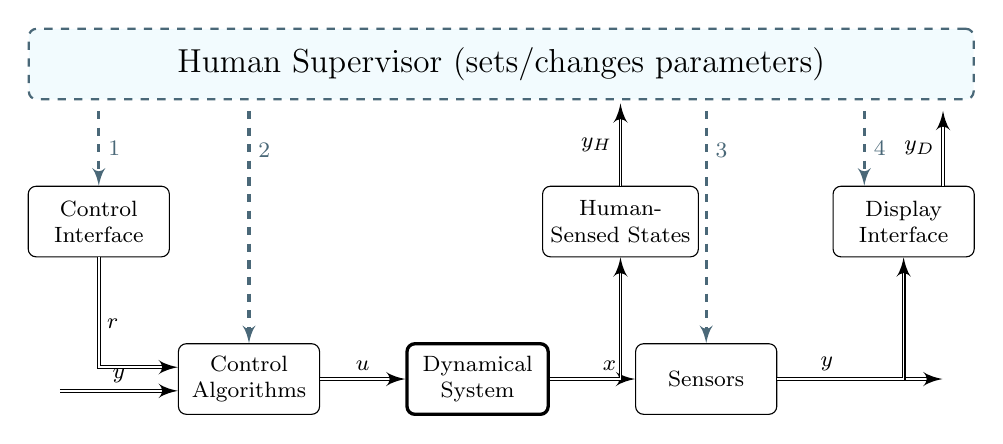
\begin{tikzpicture}[auto, node distance=2cm,>=latex'] \footnotesize
    \node at (0,0) [block, name=human, minimum width=12cm, thick, color=black!60!cyan, fill=cyan!5, text=black, dashed] {\large Human Supervisor (sets/changes parameters)};
    \node [block, below=of human.west, anchor=west] (ci) {Control\\ Interface};
    \node [block, below=of human.east, anchor=east] (di) {Display\\ Interface};
	\draw [dashed,->, very thick, color=black!60!cyan] ($(ci.north) + (0,0.95)$) -- node [pos=0.5] {$1$} (ci.north);
	\draw [dashed,->, very thick, color=black!60!cyan] ($(di.north) + (-0.5,0.95)$) -- node [pos=0.5] {$4$} ($(di.north) + (-0.5,0)$);
	\draw [double,->] ($(di.north) + (0.5,0)$) -- node [pos=0.5] {$y_D$} ($(di.north) + (0.5,0.95)$);
	
	\node at (-0.3, -4) [block, very thick] (vehicle) {Dynamical\\ System};
	\node [block, left of=vehicle, anchor=east] (ctrl) {Control\\ Algorithms};
	\node [block, right of=vehicle, anchor=west] (meas) {Sensors};
	\draw [double,->] (ctrl) -- node {$u$} (vehicle);
	\draw [double,->] (vehicle) -- node [pos=0.7] {$x$} (meas);
	\coordinate [right of=meas, node distance=3cm] (tmp3); 

	\draw [double,->] (meas.east) -- node [pos=0.3]{$y$} (tmp3);
	\draw [double,->] ($(ctrl.west) + (-1.5,-0.15)$) -- node [pos=0.5]{$y$} ($(ctrl.west) + (0,-0.15)$);

	\draw [double,->] (meas.east) -| (di.south);

	\draw [dashed,->, very thick, color=black!60!cyan] ($(meas.north) + (0,2.95)$) -- node [pos=0.17] {$3$} (meas.north);

	\draw [dashed,->, very thick, color=black!60!cyan] ($(ctrl.north) + (0,2.95)$) -- node [pos=0.17] {$2$} (ctrl.north);
	
    \node [block, left of=di, anchor=east, node distance=2.6cm] (xs) {Human-\\Sensed States};
	\draw [double,->] (xs.north) -- node [pos=0.5]{$y_H$} ($(xs) + (0,1.5)$);
	\draw [double,->] (vehicle.east) -| (xs.south);

	\draw [double,->] (ci.south) |- node [pos=0.3] {$r$} ($(ctrl.west) + (0,0.15)$);

\end{tikzpicture}

	\caption{General architecture for shared decision-making and control of complex dynamical systems, adapted from Ref.~\cite{sheridan2011adaptive}. Signals labeled $r$, $u$, $x$, and $y$ represent commands, control input, plant state, and measured plant output, respectively. The signals $y_D$ and $y_H$ represent plant output information available to the human supervisor via display interfaces and through the human's internal sensory modalities (such as the proprioceptive and vestibular systems), respectively.}
	\label{fig:sheridan_adapted}
\end{figure}

\section{Contributions}
% TODO use of "we" throughout - OK in thesis?

This thesis develops and demonstrates a shared decision-making and control architecture between humans and adaptive control algorithms. This architecture is considered in the context of flight control, where system architectures often include both supervisory human operators and autonomous flight control systems. This shared control architecture is based on the use of adaptive control algorithms to manage uncertainty in dynamics, and supervisory human operators who manage a shared response to anomalous changes in the structure of plant dynamics. This thesis will demonstrate and discuss how this shared decision-making and control architecture enables overall adaptive capabilities beyond what humans or adaptive control algorithms alone could accomplish, by making use of the benefits of collaboration between humans and adaptive control algorithms. 

This thesis is organized as follows. Chapter \ref{ch:problem} states the problem of control of a plant in the presence of parametric uncertainties as well as sudden dynamical anomalies, which are defined in more detail. Chapter \ref{ch:siso_shared_ctrl} presents the shared decision-making and control architecture in a simplified example, using control algorithms with a scalar input and access to the full plant state, and with a human pilot present on-board. Chapter \ref{ch:mimo_shared_ctrl} extends this shared decision-making and control architecture to a multi-input multi-output plant model with control design based on output feedback and remote human operators. In Chapter \ref{ch:numerical}, it is shown that the resulting shared controllers perform satisfactorily through extensive numerical simulation studies. Concluding remarks are given in Chapter \ref{ch:conclusion}.


% Problem Statement
\chapter{Problem Statement} \label{ch:problem}
% TODO (finish) describing on high level the two problems
% TODO move some details from MIMO into SISO

This thesis will consider two variations in a control problem, as described in Sections \ref{sec:siso_problem} and \ref{sec:mimo_problem}, and addressed in Chapters \ref{ch:siso_shared_ctrl} and \ref{ch:mimo_shared_ctrl}, respectively.

\section{Onboard Human Pilot and Full-State Feedback Adaptive Control} \label{sec:siso_problem}
% TODO bring notation in line with MIMO example

We consider single-input single-output (SISO) \textit{n}th-order linear dynamical plant models of the form 
\begin{equation}
\dot x_p = A_p x_p + B_p u_p	, \qquad y_p = C_p x_p \label{eq:siso_plant}
\end{equation} 
\noindent where $x_p \in \mathbb{R}^{n \times 1}$ is a state vector, and $A_p \in \mathbb{R}^{n \times n}$ and $B_p \in \mathbb{R}^{n \times 1}$ are an uncertain matrix and an uncertain vector of dynamical properties, respectively, and $u_p(t)$ is a scalar input. $C_p \in \mathbb{R}^{1 \times n}$ is a known vector producing the scalar $y_p$, the plant output, which we would like to follow prescribed commands $r(t)$ by providing a control action $u(t)$. For this problem, we consider the case where the vector $x_p$, consisting of the output $y_p$ and its first $n-1$ time derivatives, is measured and available for use in feedback control, and the vector $B_p$ is given by $B_p = [0, \cdots \, 0, \, \beta]^T$. We note that plants of this form have a transfer function from plant input to output given in the Laplace frequency domain by
\begin{equation}
\frac{Y_p(s)}{U_p(s)} = \frac{\beta}{s^n + \alpha_{n-1} s^{n-1} + \cdots + \alpha_0}	
\end{equation}
where $\alpha_i$ and $\beta$ are arbitrary coefficients. Design of the control law $u(t)$ is carried out under nominal conditions with the assumption
\begin{equation}
	u_p(t) \equiv u(t). \label{eq:siso_plant_input_nom}
\end{equation} % TODO does this form need \alpha_0 == 0?
Note that uncertainty in control effectiveness is captured by the uncertain matrix $B_p$. 

In addition to an autonomous controller which generates control input $u(t)$ in (\ref{eq:siso_plant_input_nom}), a human operator (pilot) is tasked with the high-level operation of the plant (\ref{eq:siso_plant}), including monitoring to ensure safe and anomaly-free operation. Operation is thus \textit{human-on-the-loop} as opposed to \textit{human-in-the-loop}, as the pilot does not directly command actuator input. The pilot's perceptive capabilities (as shown in Fig. \ref{fig:sheridan_adapted}) include the sensing of $y_{D} \subseteq y$, $y_{H}$, and $r$, where $y_{D}$ is a subset of vehicle sensor measurements available to the pilot through cockpit displays, $y_{H}$ is the human pilot's sensing through visual and vestibular modalities, and $r$ is the prescribed command for plant output.

% TODO here and MIMO sec, change "no role in feedback control"

%An adaptive autopilot based on model reference adaptive control (MRAC) is capable of addressing anomalies that can be represented as parametric uncertainties, but may perform poorly when an anomaly causes the order of the vehicle dynamics to change \cite{narendra2012stable, lavretsky2013robust}. A human pilot flying manually may detect such an anomaly and adapt to the anomalous dynamics, but the pilot's tracking performance may be noticeably poorer after a change in dynamics and pilot adaptation \cite{hess2015modeling, zaal2016manual}. 

% TODO remove "case (x)" notation everywhere
We consider the introduction of two severe anomalies in the dynamics of the plant model (\ref{eq:siso_plant}), described in Sections \ref{subsec:siso_act_fault} and \ref{subsec:siso_delay}. The first consists of a change in the actuator dynamics, represented as a change in the actuator model from a gain to a first-order lag. The second anomaly is a latency introduced in the feedback of state information to the control algorithms. 

% TODO move paragraph on assumptions of what human pilot has access to here

%The remote human supervisor has information on plant sensor measurements, state estimate, tracking performance, and health (via visual, haptic, and/or auditory interfaces). \textit{Human-in-the-loop} operation is possible via remote controls, allowing the operator to actuate the plant by manually providing $u(t)$ in (\ref{eq:first_order_act}) and (\ref{eq:second_order_act}). The sensing and actuation by the remote human supervisor include time delays $\tau_s, \tau_a > 0$, respectively.

The problem we investigate in Chapter \ref{ch:siso_shared_ctrl} is whether we can use a suitable combination of 
\begin{enumerate}[label=(\alph*)]
	\item autonomous control methodologies
	\item an onboard human pilot
\end{enumerate}
to successfully mitigate the two types of anomalous dynamics to be described presently and restore tracking performance in the presence of uncertainty. We refer to this class of anomaly response as a shared control response. This work builds on anomaly response frameworks using adaptive autopilots and on-board human pilots reported in \cite{farjadian2017bumpless} as well as the shared controller in Chapter \ref{ch:siso_shared_ctrl} of this thesis.

% TODO probably remove self-citation in thesis?

\subsection{Actuator Fault} \label{subsec:siso_act_fault}
An anomaly is introduced which changes the actuator dynamics from a direct input (\ref{eq:siso_plant_input_nom}) to a first-order lag
\begin{equation}
	T_L\dot{u}(t) + u(t) = u_p(t) \label{eqn:actuator_dynamics_symbolic}
\end{equation} 
\noindent so that the dynamics of plant augmented with actuator dynamics change suddenly from order $n$ to order $n+1$. We can define an augmented plant 
\begin{equation}
	\dot{x}_p' = A_p' x_p' + B_p' u	\label{eqn:plant_3_compact}
\end{equation}
where $u(t)$ is defined in (\ref{eqn:actuator_dynamics_symbolic}), and $x_p'$ consists of the output $y_p$ and its first $n$ time derivatives. The matrix $A_p'$ and vector $B_p'$ are then given by
\begin{equation}
	A_p' = \begin{bmatrix}
		\begin{matrix}0 \\ \vdots \end{matrix} & \Bigg[ \quad I_n \quad ~ \Bigg] \\ \alpha_0' & \begin{matrix}\cdots & \alpha_{n+1}' \end{matrix}
	\end{bmatrix}, \quad B_p' = \begin{bmatrix}
		0 \\ \vdots \\ \beta'
	\end{bmatrix}
	\label{eqn:plant_3_symbolic}
\end{equation}
%\begin{equation}
%	\underbrace{\begin{bmatrix}
%		\dot{\phi} \\ \dot{p} \\ \ddot{p}
%	\end{bmatrix}}_{\dot{x}_p'} = \underbrace{\begin{bmatrix}
%		0 & 1 & 0\\ 0 & 0 & 1 \\ 0 & \frac{L_p}{T_L} & L_p - \frac{1}{T_L}
%	\end{bmatrix}}_{A_p'} \underbrace{\begin{bmatrix}
%		\phi \\ p \\ \dot{p}
%	\end{bmatrix}}_{x_p'} + \underbrace{\begin{bmatrix}
%		0 \\ 0 \\ \frac{L_{\delta_a}}{T_l}
%	\end{bmatrix}}_{B_p'} u
%	\label{eqn:plant_3_symbolic}
%\end{equation}
where $I_n$ is the identity matrix of dimension $n$ and $\alpha_i', \, \beta'$ are uncertain coefficients. If the change in the order of the plant is not known to the adaptive controller, it may no longer be possible for it to stabilize the plant following such a change. The question then is if a shared decision-making architecture, with suitable action from the human pilot leading to feedback on the augmented state vector $x_p'$, can result in the recovery of closed-loop performance with anomalous actuator model (\ref{eqn:actuator_dynamics_symbolic}).

\subsection{Time-Delayed Sensor Measurements} \label{subsec:siso_delay}
We consider the introduction an anomaly in the cyber-physical space consisting of the dynamical system with feedback control via adaptive control algorithms, which leads to latency in the feedback of plant state information. We model this anomaly as the addition of a time delay $\tau$ of the state measurements before the computation of the control input, causing a discrepancy between the plant state $x_p$ and the state as sensed by the controller, denoted $x_\sigma$, given by
\begin{equation}
	x_\sigma(t) = x_p(t - \tau). \label{eqn:delay_approx_diffeq}
\end{equation}

We note that the time delay $\tau$ may be approximated up to a certain frequency as a first-order filter, given in the Laplace frequency domain as
\begin{equation}
	e^{-\tau s} \approx \frac{1}{1 + \tau s}.
\end{equation}
In the time domain, this approximation corresponds to the differential equation
\begin{equation}
	\tau \dot{x}_{\sigma}(t) + x_{\sigma}(t) \approx x_p(t)	
\end{equation}

We note that this effectively increases the order of the plant from $n$ to $n+1$ when we consider the output to be the delayed signal. In this case, using the time delay approximation of (\ref{eqn:delay_approx_diffeq}), the augmented plant model is given by
\begin{equation}
	\dot{x}_\sigma' = A_p' x_\sigma' + B_p' u \label{eqn:plant_3_tau}
\end{equation}
with $A_p'$ and $B_p'$ defined in (\ref{eqn:plant_3_symbolic}). Due to this similarity, we investigate the applicability of a shared control solution to the problem of Section \ref{subsec:siso_act_fault} to the problem of a time-delayed state measurement. The shared control architecture which we propose for these two problems is presented in Chapter \ref{ch:siso_shared_ctrl}.

%\begin{equation}
%	\underbrace{\begin{bmatrix}
%		\dot{\phi} \\ \dot{p} \\ \ddot{p}
%	\end{bmatrix}}_{\dot{x}_\sigma'} = \underbrace{\begin{bmatrix}
%		0 & 1 & 0\\ 0 & 0 & 1 \\ 0 & \frac{L_p}{\tau} & L_p - \frac{1}{\tau}
%	\end{bmatrix}}_{A_\sigma'} \underbrace{\begin{bmatrix}
%		\phi \\ p \\ \dot{p}
%	\end{bmatrix}}_{x_\sigma'} + \underbrace{\begin{bmatrix}
%		0 \\ 0 \\ \frac{L_{\delta_a}}{\tau}
%	\end{bmatrix}}_{B_\sigma'} u
%	\label{eqn:plant_3_tau}
%\end{equation}

\section{Remote Human Operation and Output Feedback Adaptive Control}  \label{sec:mimo_problem}
Here we consider the problem of controlling linear multi-input multi-output (MIMO) plant models of the form
\begin{equation}
\begin{gathered}
\dot x_p = (A_p + B_p \Theta_p^T) x_p + B_p \Lambda_p u_p \\
y_p = C_p x_p, \qquad z_p = C_{pz} x_p \label{eq:plant_dynamics}
\end{gathered}
\end{equation}
where $x_p$ is the plant state, $u_p$ is the plant input, $y_p$ is measured output, and $z_p$ is regulated output. Uncertain dynamics lead to the introduction of unknown $\Theta_p$ and $\Lambda_p$ in the plant model. It is assumed that the matrix $CB$ has full rank, and thus the plant has uniform relative degree one (see \cite{qu2016adaptive}). In addition to the dynamics (\ref{eq:plant_dynamics}), the plant's actuators have the first-order dynamics
\begin{equation}
	\dot{u}_p + (D_1 + \Theta_1^T) u_p = D_1 u \label{eq:first_order_act}
\end{equation}
where $D_1$ is a diagonal matrix representing nominal actuator parameters and $\Theta_1$ models uncertainty in the actuator dynamics. The problem is to choose $u(t)$ such that $z_p(t)$ tracks an external command $z_{cmd}(t)$ as closely as possible.
%Model reference adaptive control (MRAC) with output feedback and closed-loop reference models, such as the method of \cite{qu2016adaptive}, can achieve asymptotic tracking and guarantee stability for this control problem. 

\subsection{Actuator Fault} \label{subsec:mimo_act_fault}
Consider the occurrence of an anomaly which causes an abrupt change in actuator dynamics from (\ref{eq:first_order_act}) to the second-order model
\begin{equation}
	\ddot{u}_p + (D_2 + \Theta_2^T) \dot{u}_p + (D_1 + \Theta_1^T) u_p = D_1 u \label{eq:second_order_act}
\end{equation}
where in addition to $\Theta_1$, $\Theta_2$ is an unknown parameter as well. This change in dynamics means that the the structure of the model used for control design is no longer accurate, and the autonomous controller may lose stability and command tracking ability. In particular, the challenge from the anomaly is the increase in relative degree between $u$ and $y_p$ from two to three.

In addition to an autonomous controller which generates control input $u(t)$ in (\ref{eq:first_order_act}) and (\ref{eq:second_order_act}), a human supervisor is tasked with the high-level operation of the plant (\ref{eq:plant_dynamics}), including mission and task planning (commanding its mode of operation) and monitoring to ensure safe and anomaly-free operation. In this chapter, we consider \textit{remote} human operators who cannot sense the vehicle state and dynamics directly through vestibular pathways. The human supervisor may be responsible for the supervision of multiple plant instances, as illustrated in Fig. \ref{fig:uav_supervisor} for the case of HALE VFA platforms. Operation is considered \textit{human-on-the-loop} in the same manner as the onboard human pilot considered in the problem of Chapter \ref{sec:siso_problem}. 

\begin{figure}[htbp]
	\centering
	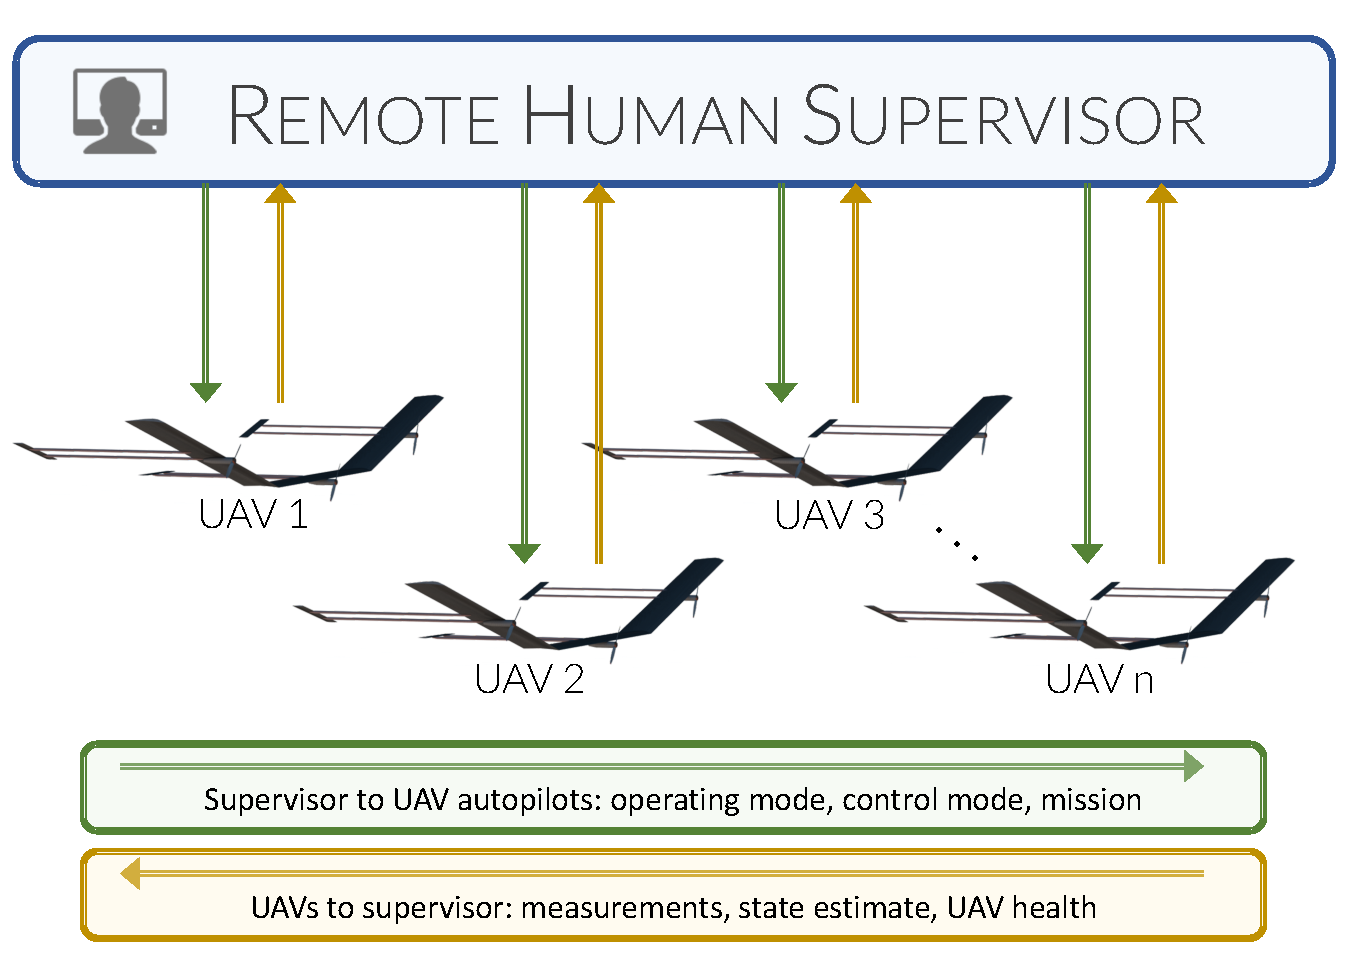
\includegraphics[width=0.95\columnwidth]{uav_supervisor.pdf}
	\caption{Supervisory operation of a fleet of HALE UAVs}
	\label{fig:uav_supervisor}
\end{figure}

It is assumed that the human supervisor has access to information on plant sensor measurements, state estimate, tracking performance, and health (via visual, haptic, and/or auditory interfaces), and is able to perceive changes in plant dynamics, such as an increased lag or decreased control effectiveness, via these interfaces.  \textit{Human-in-the-loop} operation is possible via remote controls, allowing the operator to actuate the plant by manually providing $u(t)$ in (\ref{eq:first_order_act}) and (\ref{eq:second_order_act}). The sensing and actuation by the remote human supervisor include time delays $\tau_s, \tau_a > 0$, respectively.

The problem we investigate in Chapter \ref{ch:mimo_shared_ctrl} is whether the design of $u(t)$ can be carried out using a shared decision-making and control architecture using
\begin{enumerate}[label=(\alph*)]
	\item autonomous control methodologies
	\item a remote human supervisor
\end{enumerate}
so as to lead to a successful mitigation of an abrupt anomaly causing a change from (\ref{eq:first_order_act}) to (\ref{eq:second_order_act}) and restore tracking performance in the presence of uncertainty.
  
%  We refer to this class of anomaly response as a shared control response. This work builds on anomaly response frameworks using adaptive autopilots and on-board human pilots reported in \cite{farjadian2017bumpless} and \cite{thomsen2018shared}.

% TODO work in some motion planning / robotics refs somewhere
\chapter{Shared Control with Human Pilot and State Feedback} \label{ch:siso_shared_ctrl}
%%%%%%%%%%%%%%%%%%%%%%%%%%%%%%%%%%%%%%%%%%%%%%%%%%%%%%%%%%%%%%%%%%%%%%%%%%%%%%%%

In this chapter, we introduce a shared control architecture between human pilots and adaptive control algorithms to address the problems defined in Section \ref{sec:siso_problem}. Adaptive controllers can be designed to permit autonomous control of the vehicle (\ref{eq:siso_plant}) in the presence of parametric uncertainties in $A_p$ and $B_p$. On-board human pilots monitor the performance of the vehicle and are trained to manually control the vehicle in case of autopilot failure. Our shared anomaly response tasks the human pilot with providing key inputs based on higher-level perception of the anomaly, but delegates the low-level regulation and command tracking tasks to adaptive control algorithms which make use of these inputs. In Section \ref{sec:siso_sc_adaptive}, we describe two adaptive autopilot designs which in combination with the human operator whose precise role is described subsequently in Section \ref{sec:siso_sc_human}, will solve the problem which was presented in Section \ref{sec:siso_problem}. The overall shared control architecture is summarized in Section \ref{sec:siso_sc_overall}.

\section{Adaptive Autopilot} \label{sec:siso_sc_adaptive}
Central to this work is the use of an autopilot which employs advanced control principles for low-level flight control tasks in the place of human pilots. In particular, our autopilot design uses adaptive control with vehicle states available for feedback \cite{narendra2012stable}. Closed-loop reference models (CRMs) \cite{gibson2013adaptive} are utilized here to improve the transient performance of adaptive control, in comparison to open-loop reference models.

In this section, a \textit{nominal} adaptive controller is designed to allow tracking of commands for the \textit{n}th-order linear dynamical system given in (\ref{eq:siso_plant}). A \textit{recovery} adaptive controller is then designed for the (\textit{n+1})th-order system given in (\ref{eqn:plant_3_compact}) which arises following an anomaly that changes the system dynamics.

\subsection{Nominal Adaptive Controller}
The adaptive controller described in this section will be designed so as to produce a control input $u(t)$ to the plant (\ref{eq:siso_plant}), of the form
\begin{equation}
	u(t) = \theta(t) x_p(t) + q(t) r(t)
	\label{eqn:control_law}
\end{equation}
\noindent where $\theta(t) \in \mathbb{R}^{1 \times n}$ is a vector of adaptive feedback gains on the plant state vector, and $q(t)$ is a scalar adaptive feedforward gain on the external reference input (command), $r(t)$. The gains $\theta(t)$ and $q(t)$ will be adjusted online so that desired closed-loop command following behavior is achieved in the presence of uncertain plant parameters. The design of the adaptive controller is based upon the dynamics of a reference model, a dynamical system given by
\begin{equation}
	\dot{x}_m(t) = A_m x_m(t) + B_m r(t) - L_m \left[x_p(t) - x_m(t)\right]
	\label{eqn:crm}
\end{equation}
\noindent where $A_m \in \mathbb{R}^{n \times n}$ is Hurwitz, $B_m \in \mathbb{R}^{n \times 1}$, $L_m \in \mathbb{R}^{n \times n}$, and $e(t) \equiv x_p(t) - x_m(t)$ is defined as the state error. The matrix $A_m$ can be designed using techniques such as the linear quadratic regulator (LQR) method to model a desired closed-loop system dynamic response (i.e. $A_m = \hat{A}_p + \hat{B}_p K_{lqr}$, where $\hat{A}_p$ and $\hat{B}_p$ are known approximations of uncertain $A_p$ and $B_p$). It is assumed that there exists scalar $\lambda$ such that $B_p \equiv \lambda B_m$. The matrix $L_m \neq 0$ differentiates this closed-loop reference model from an open-loop reference model. 

With the plant, control law, and reference model dynamics defined in (\ref{eq:siso_plant}), (\ref{eqn:control_law}), and (\ref{eqn:crm}), respectively, feedback gain $\theta^*$ and feedforward gain $q^*$ are defined by the following relations
\begin{eqnarray}
	A_p + B_p \theta^* &=& A_m \label{eqn:matchcond1} \\
	B_p q^* &=& B_m \label{eqn:matchcond2} 
\end{eqnarray}
and it is noted that when $\theta(t) = \theta^*$ and $q(t) = q^*$, the closed-loop dynamics of the plant will match that of the reference model. These relations are denoted as the matching conditions of the adaptive controller.

Feedback and feedforward control gain adaptation is given by the adaptive laws
\begin{eqnarray}
	\dot{\theta}(t) &=& - \Gamma_\theta B_m^T P e(t) x_p^T(t) \label{eqn:adaptive_law_theta}\\
	\dot{q}(t) &=& - \gamma_q B_m^T P e(t) r(t)
	\label{eqn:adaptive_law_gamma}
\end{eqnarray}
\noindent where $\Gamma_\theta > 0$ and $\gamma_q > 0$ are a diagonal matrix and scalar, respectively, of constant weights. These weights correspond to learning rates on the feedback/feedforward parameters. The state error feedback gain, $L_m$, can be chosen to be
\begin{equation}
	L_m = - A_m - \Gamma_\theta
	\label{eqn:L_m}
\end{equation}
\noindent which ensures that there exists positive definite matrix $P > 0$, the solution to the Lyapunov equation 
\begin{equation}
(A_m + L_m)^T P + P(A_m + L_m) = - Q
\end{equation}
for any positive definite matrix $Q > 0$. 

% change notation to match text
\begin{figure}[t]
	\centering
	
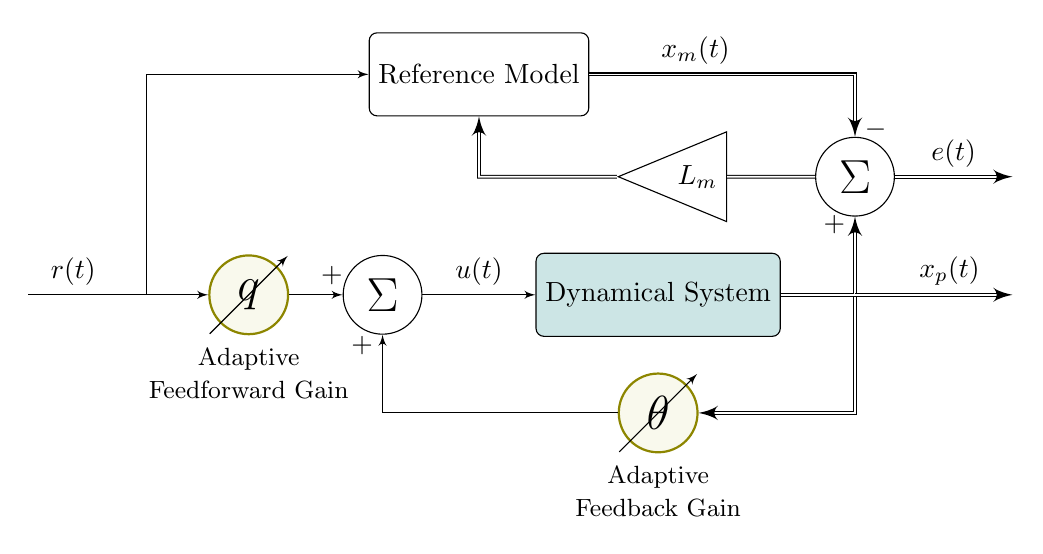
\begin{tikzpicture}[auto, node distance=2cm,>=latex']
    \node [input, name=input] {};
    \coordinate [name=input_inter, right of=input, node distance=1.5cm];
    \node [gain, right of=input_inter, node distance=1.3cm] (ff) {\LARGE $q$};
    \coordinate [below left of=ff, node distance=0.7cm] (ff_bl);
    \coordinate [above right of=ff, node distance=0.7cm] (ff_ar);
    \draw [->] (ff_bl) -- (ff_ar);
    
    \node [align=center, below of = ff, node distance=1cm] {\small Adaptive\\\small Feedforward Gain};
    \node [sum, right of=ff, node distance=1.7cm] (sum) {\LARGE $\Sigma$};
%    \node [block, right of=sum] (controller) {Controller};
    \node [block, right of=sum, 
            node distance=3.5cm, fill=blue!50!green!20] (system) {Dynamical System};
%    \node [block, right of=rm, node distance=4cm] (adaptive){Adaptive Law};
	\node [gain, below of=system] (fb) {\LARGE $\theta$};
    \coordinate [below left of=fb, node distance=0.7cm] (fb_bl);
    \coordinate [above right of=fb, node distance=0.7cm] (fb_ar);
    \draw [->] (fb_bl) -- (fb_ar);

    \node [align=center, below of = fb, node distance=1cm] {\small Adaptive\\\small Feedback Gain};

    \draw [->] (sum) -- node[name=u] {$u(t)$} (system);
    \coordinate [name=output_inter, right of=system, node distance=2.5cm];
    \node [output, right of=output_inter] (output) {};
%    \coordinate [below of=u] (tmp);

    \draw [draw,->] (input) -- node [pos=0.25] {$r(t)$} (ff);
    \draw [draw,->] (ff) -- node [pos=0.8] {$+$} (sum);
%    \draw [->] (sum) -- node {$e(t)$} (controller);
%    \draw [double,->] (system) -- node [near end] {$x_p(t)$} (output);
%    \draw [->] (y) |- (tmp) -| node[pos=0.99] {$+$} 
%        node [near end] {$y_m(t)$} (sum);
    \draw [double,->] (output_inter) |- (fb);
    \draw [draw,->] (fb) -| node[pos=0.93] {$+$} (sum);
    	
    \node [sum, above of=output_inter] (sum_e) {\LARGE $\Sigma$};
    \draw [double,->] (system) -|  node [pos=0.95] {$+$} (sum_e);
    \draw [double,->] (output_inter) --  node [pos=0.6] {$x_p(t)$} (output);
%    \coordinate [name=err_mid, left of = sum_e, node distance=1cm];
    \coordinate [name=err_end, right of = sum_e];
	\draw [double,->] (sum_e) -- node [pos=0.5] {$e(t)$} (err_end);
		
    \node [block, above of=u, node distance = 2.5cm] (rm){Reference Model};
    \draw [->] (input_inter) |- (rm);
    \draw [double,->] (rm) -| node [pos=0.2] {$x_m(t)$} node [pos=0.94] {$-$} (sum_e);

	\node [tri_gain, left of=sum_e] (lm) {$L_m$};
%	\coordinate [left of=rm, node distance=2cm] (err_fb);
	\draw [double,->] (sum_e) -- (lm) -| (rm);

\end{tikzpicture}

	\caption{Block diagram of model reference adaptive controller with closed-loop reference model}
	\label{fig:mrac_block}
\end{figure}

To ensure robustness of the adaptive controller, a projection operator \cite{pomet1992adaptive, lavretsky2011projection} may be used in conjunction with the adaptive laws (\ref{eqn:adaptive_law_theta}) and (\ref{eqn:adaptive_law_gamma}). The projection operator limits the magnitude of $\dot{\theta}(t)$ and $\dot{q}(t)$, so that the parameters $\theta(t)$ and $q(t)$ remain within a convex set. Readers are referred to Ref.~\cite{gibson2013adaptive} for a detailed treatment of the projection operator as it applies to the general CRM-adaptive controller, but to summarize, the adaptive laws are modified from (\ref{eqn:adaptive_law_theta}) and (\ref{eqn:adaptive_law_gamma}) to be
\begin{eqnarray}
	\dot{\theta}(t) &=& \text{Proj}(- \Gamma_\theta B_m^T P e(t) x_p^T(t),\text{ } \theta(t)) \label{eqn:thetadot_projection} \\
	\dot{q}(t) &=& \text{Proj}(- \gamma_q B_m^T P e(t) r(t),\text{ } q(t)) \label{eqn:qdot_projection}
\end{eqnarray}
\noindent with the vector projection operator defined as
\begin{equation}
	\text{Proj}(Y, \Phi) = \left[ \text{Proj}(y_1, \varphi_1) \ldots \text{Proj}(y_n, \varphi_n) \right]
\end{equation}
\noindent and the scalar projection operator defined as
\begin{equation}
	\text{Proj}(y, \varphi) = \begin{cases}
		y(1 - f(\varphi)) & f(\varphi) > 0 \land y \nabla f(\varphi) > 0\\
		\hfil y & \text{otherwise}
	\end{cases}
\end{equation}

\noindent The function $f(\varphi)$ is taken to be
\begin{equation}
	f(\varphi) = \frac{\varphi^2 - \varphi_{m}^2}{2 \varphi_{\epsilon} \varphi_{m} + \varphi_{\epsilon}^2}
	\label{eqn:proj_function}
\end{equation}
\noindent where $\varphi_{m}$ and $(\varphi_{m} + \varphi_{\epsilon})$ define ``soft'' and ``hard'' bounds on the parameter $\varphi$, respectively. 

With a plant given by (\ref{eq:siso_plant}), a control law defined as in (\ref{eqn:control_law}), a reference model as in (\ref{eqn:crm}), and parameter adaptation as in (\ref{eqn:thetadot_projection}) and (\ref{eqn:qdot_projection}), the goal of command tracking in the presence of parametric uncertainties is achieved. Section \ref{subsec:siso_recovery_ac} describes a modification to the adaptive control design introduced in this section, which will constitute a portion of the shared control response to anomalies, as described in Chapter \ref{sec:siso_problem}.

\subsection{Recovery Adaptive Controller} \label{subsec:siso_recovery_ac}
The \textit{recovery} adaptive controller here is designed using the same methods as that of the \textit{nominal} adaptive controller described above, however it is designed based on a higher-order model of the plant, which is defined in (\ref{eqn:plant_3_symbolic}). In order to satisfy the matching conditions for adaptive control given in (\ref{eqn:matchcond1}) and (\ref{eqn:matchcond2}), a corresponding higher-order reference model, accommodating additional state information, must be designed. The control law has the form
\begin{equation}
	u(t) = \theta(t) x_p'(t) + q(t) r(t)
	\label{eqn:control_law_3}
\end{equation}
where $x_p' \in \mathbb{R}^{n+1 \times 1}$ is the state of the plant augmented with first-order actuator dynamics, as in (\ref{eqn:plant_3_symbolic}). The closed-loop reference model is then given by
\begin{equation}
	\dot{x}_m'(t) = A_m' x_m'(t) + B_m' r(t) - L_m' \left[x_p'(t) - x_m'(t)\right].
	\label{eqn:crm_3}
\end{equation}
With a plant given by (\ref{eqn:plant_3_symbolic}), a control law defined as in (\ref{eqn:control_law_3}), a reference model as in (\ref{eqn:crm_3}), and parameter adaptation designed identically to (\ref{eqn:thetadot_projection}) and (\ref{eqn:qdot_projection}) in the augmented state space, command tracking in the presence of parametric uncertainties is achieved for the plant with first-order actuator dynamics (\ref{eqn:plant_3_symbolic}). This adaptive controller is referred to as the recovery adaptive controller, as it will be used in conjunction with a human pilot in the proposed shared control framework to recover from dynamical anomalies.

\section{Human Pilot} \label{sec:siso_sc_human}
Trained human pilots develop interal models of the vehicle dynamics and expected performance in different situations, giving pilots a high level of situation awareness regarding the aircraft \cite{endsley1995toward}. The idea is to task the human pilot with responsibilities which require a high level of cognition in the shared response to an anomaly, in order to allow the use of the recovery adaptive autopilot described in Section \ref{subsec:siso_recovery_ac} for low-level regulation and command tracking tasks following the anomaly. 

The role of the human pilot in the shared controller is described as follows, as a sequence of responsibilities following the occurrence of an anomaly.
\begin{enumerate}[label=\textbf{Task \arabic*.}, leftmargin=1.8cm]
	\item Timely detection of anomalous closed-loop dynamical behavior
	\item Characterization of anomaly
	\item Commanding a change from nominal autopilot to recovery autopilot
\end{enumerate}

The time when the anomaly occurs is denoted $t := t_1^*$, the time when the pilot completes the final task is denoted $t := t_2^*$, and the time at which irrecoverable failure is reached without the pilot completing all tasks is denoted $t := t_3^*$. The human pilot must complete Tasks 1--3 such that $t_2^* < t_3^*$ if a recovery is to be successful.

Completion of the first task requires that the on-board human pilot is able to perceive that something is wrong with the vehicle dynamics, and that deterioration in closed-loop performance is not caused by external disturbances or transient behavior in adaptation to changing parameters.

The second tasks requires the human pilot to understand more about the nature of the anomaly. For the anomaly considered in Section \ref{subsec:siso_act_fault}, the pilot must perceive the additional lag in response to control inputs caused by the actuator anomaly. Even in a human-on-the-loop situation, when the pilot is not directly responsible for the generation of control input $u(t)$, anomalous vehicle behavior is expected to be manifested through changes in the closed-loop response of the vehicle and its disturbance-rejection abilities. Additionally, it is assumed that the pilot is able to perceive the autopilot's control actions, $u(t)$, through visual displays or through kinesthetic or tactile feedback on the pilot's controls \cite{tan1994human, yang2007development}. In combination with the pilot's visual and vestibular sensing of vehicle dynamics, this sensing of autopilot control actions will allow the human pilot to determine the open-loop vehicle dynamics, in addition to the closed-loop dynamics, allowing for an enhanced perception and understanding of an anomaly. In the case of the anomaly considered in Section \ref{subsec:siso_delay}, the time-delayed sensor measurements would change the relationship between $y_{H}$ and $y_{D}$, in addition to the closed-loop vehicle dynamics. 

The final task involves the transfer of the pilot's diagnosis to the autopilot, by changing the autopilot from its nominal adaptive control mode to the recovery adaptive control mode. We therefore hypothesize that an on-board human pilot has the sensory and perceptive capabilities necessary -- with proper training -- to carry out Tasks 1--3 in the presence of the anomalies described in Section \ref{sec:siso_problem}. 

\section{Overall Shared Controller}\label{sec:siso_sc_overall}

The shared control algorithm between the adaptive autopilot and human pilot that we propose is as follows. Under nominal operating conditions, the adaptive controller as in (\ref{eqn:control_law}), (\ref{eqn:thetadot_projection}), and (\ref{eqn:qdot_projection}) is proposed. An anomaly is assumed to occur at $t=t_1^*$. Following this time instant, the pilot carries out Tasks 1--3 as in Section \ref{sec:siso_sc_human}, and at $t=t_2^*$ indicates to the adaptive autopilot the perceived increase in order. Using this pilot input, we propose an adaptive controller predicated on a higher-order dynamics of the open-loop plant (the recover adaptive controller) and assume that in addition to the plant output and its first $n-1$ time derivatives, the $n$th derivative with respect to time is measurable. 

\begin{figure}[h]
	\centering
	
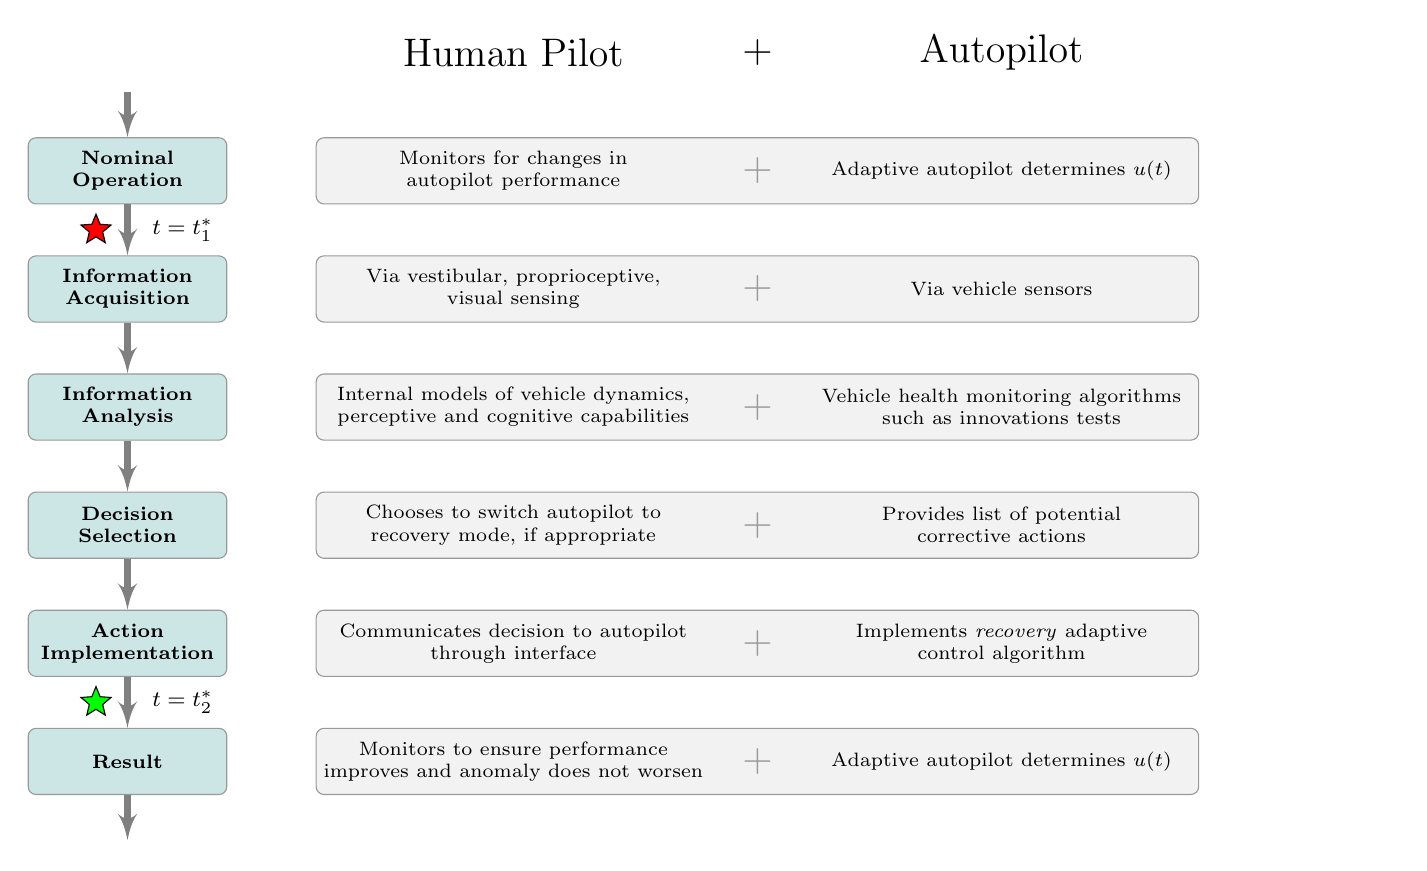
\begin{tikzpicture}[auto, node distance=1.5cm,>=latex'] \scriptsize
    \node (hp) at (0,0) {\Large Human Pilot};
    \node (p1) at (3.1,0) {\Large $+$};
    \node (ap) at (6.2,0) {\Large Autopilot};
    
    \node [row, below of = p1] (r1) {\Large $+$};
    \node [row, below of = r1] (r2) {\Large $+$};
    \node [row, below of = r2] (r3) {\Large $+$};
    \node [row, below of = r3] (r4) {\Large $+$};
    \node [row, below of = r4] (r5) {\Large $+$};
    \node [row, below of = r5] (r6) {\Large $+$};
    
    \node [stage, left of = r1] (s1) {\scriptsize Nominal\\\scriptsize Operation};
    \node [stage, left of = r2] (s2) {\scriptsize Information\\\scriptsize Acquisition};
    \node [stage, left of = r3] (s3) {\scriptsize Information\\\scriptsize Analysis};
    \node [stage, left of = r4] (s4) {\scriptsize Decision\\\scriptsize Selection};
    \node [stage, left of = r5] (s5) {\scriptsize Action\\\scriptsize Implementation};
    \node [stage, left of = r6] (s6) {\scriptsize Result};
    
	\node[star, fill=red, minimum width=0.4cm, inner sep=0pt, star points=5, star point ratio=2.25, draw] (anom) at (-5.3,-2.25) {};
	\node [right of = anom, node distance = 1.1cm] {\footnotesize $t = t_1^*$};
	
	\node[star, fill=green, minimum width=0.4cm, inner sep=0pt, star points=5, star point ratio=2.25, draw] (fix) at (-5.3,-8.25) {};
	\node [right of = fix, node distance = 1.1cm] {\footnotesize $t = t_2^*$};

    \draw [arr] ($(s1)+(0,1)$) -- (s1);
    \draw [arr] (s1) -- (s2);
    \draw [arr] (s2) -- (s3);
    \draw [arr] (s3) -- (s4);
    \draw [arr] (s4) -- (s5);
    \draw [arr] (s5) -- (s6);
    \draw [arr] (s6) -- ($(s6)+(0,-1)$);
        
	\node [note, below of = hp] (hp1) {\scriptsize Monitors for changes in\\\scriptsize autopilot performance};
	\node [note, below of = hp1] (hp2) {\scriptsize Via vestibular, proprioceptive, \\\scriptsize visual sensing};
	\node [note, below of = hp2] (hp3) {\scriptsize Internal models of vehicle dynamics, \\\scriptsize perceptive and cognitive capabilities};
	\node [note, below of = hp3] (hp4) {\scriptsize Chooses to switch autopilot to\\\scriptsize recovery mode, if appropriate};
	\node [note, below of = hp4] (hp5) {\scriptsize Communicates decision to autopilot\\\scriptsize through interface};
	\node [note, below of = hp5] (hp6) {\scriptsize Monitors to ensure performance \\\scriptsize improves and anomaly does not worsen};
	
	\node [note, below of = ap] (ap1) {\scriptsize Adaptive autopilot determines $u(t)$};
	\node [note, below of = ap1] (ap2) {\scriptsize Via vehicle sensors};
	\node [note, below of = ap2] (ap3) {\scriptsize Vehicle health monitoring algorithms\\\scriptsize such as innovations tests};
	\node [note, below of = ap3] (ap4) {\scriptsize Provides list of potential\\\scriptsize corrective actions};	
	\node [note, below of = ap4] (ap5) {\scriptsize Implements \textit{recovery} adaptive\\\scriptsize control algorithm};
	\node [note, below of = ap5] (ap6) {\scriptsize Adaptive autopilot determines $u(t)$};
\end{tikzpicture}

	\caption{Proposed framework for shared decision-making and control following an anomaly, with stages of decision making categorized in Ref.~\cite{parasuraman2000model}}
	\label{fig:response_flow}
\end{figure}

For the case of an actuator anomaly as in (\ref{eqn:actuator_dynamics_symbolic}), $\theta^* \in \mathbb{R}^3$ and $q^*$ exist that solve the corresponding matching conditions in (\ref{eqn:matchcond1}) and (\ref{eqn:matchcond2}), and an adaptive controller as in (\ref{eqn:thetadot_projection}) and (\ref{eqn:qdot_projection}) can be realized to lead to a stable closed-loop solutions and accurate tracking. These matching conditions are not met, however, in the case of the anomaly causing time-delayed sensor measurements (\ref{eqn:delay_diffeq}). In the numerical examples, we will discuss the details of how such an adaptive controller with an increase in dimension following the pilot input performs for both cases of anomalies. 

A detailed discussion of the stability of the resulting adaptive controller is not carried out in this thesis. But it is clear that if the time period ($t_2^* - t_1^*$) is sufficiently short compared to ($t_3^* - t_1^*$), the adaptive controller will guarantee boundedness of the closed-loop system and convergence of $e(t)$ to zero if our assumptions that the cause of the two anomalies results in an $(n+1)$-order plant and that its states are measurable are satisfied. Thus, if the human pilot carries out Tasks 1--3 sufficiently fast, the anomaly response based on this shared control architecture will restore closed-loop performance and stability in the presence of a sustained anomaly. We carry out detailed numerical simulation studies in Chapter \ref{ch:numerical} and evaluate the performance of this proposed shared control architecture in response to dynamical anomalies.

% Shared Control
\chapter{Shared Control with Remote Human Pilot and Output Feedback}  \label{ch:mimo_shared_ctrl}
The shared control framework we propose is designed so as to combine the merits of both adaptive control algorithms and remote human operators. Adaptive autopilots and complementary higher-level motion planning algorithms allow for continuous autonomous operation of the vehicle in the presence of parametric uncertainties $\Theta_p$, $\Lambda_p$, and $\Theta_1$. Remote human operators monitor the performance of the vehicles and are trained and able to remotely pilot the vehicle in case of autopilot failure. The remote piloting of the vehicles, however, is a daunting task due to communication delays and a weakened understanding of the vehicle dynamics, state, and environment, due to the remote nature of the task. Our shared anomaly response tasks the human operator with providing key inputs based on higher-level perception of the anomaly, but delegates the low-level regulation and command tracking tasks to adaptive control algorithms which make use of these inputs. In Section \ref{subsec:sc_adaptive}, we describe two adaptive autopilot designs which in combination with the human operator whose precise role is described subsequently in Section \ref{subsec:sc_human}, will solve the problem which was presented in Section \ref{sec:mimo_problem}. The overall shared control architecture is summarized in Section \ref{subsec:sc_overall}.

% TODO merge all edits from CPHS paper
% TODO add LQR cost function in order to give numerical values
% TODO get rid of quotes on nominal, recovery
\section{Adaptive Output-Feedback Control}\label{subsec:sc_adaptive}
An autonomous controller is designed to track prescribed commands for plant outputs $z_p(t)$ in (\ref{eq:plant_dynamics}). The shared control framework involves separate adaptive control designs for the plant (\ref{eq:plant_dynamics}) in combination with actuator dynamics (\ref{eq:first_order_act}) and (\ref{eq:second_order_act}). The control design accommodating first-order actuators is denoted the \textit{nominal} adaptive control design, and excluding exceptional failures, is the controller in use by the autopilot. The control design accommodating second-order actuators is a predefined \textit{recovery} adaptive controller, whose use case will be defined more fully in Section \ref{subsec:sc_human}. To achieve the control goals stated in Section \ref{ch:problem}, control design consists of
\begin{enumerate}[label=(\roman*)]
	\item baseline control design using the robust servomechanism linear quadratic regulator method (RSLQR);
	\item adaptive output-feedback augmentation for parametric uncertainties in the plant.
\end{enumerate}

Control design in each case uses an augmented linear plant formulation, where the plant (\ref{eq:plant_dynamics}) is extended with the actuator dynamics -- either (\ref{eq:first_order_act}) or (\ref{eq:second_order_act}) -- as well as integrated tracking errors 
\begin{equation}
	e_z^{\mathcal{I}}(t) = \int_0^{t} \big( z_p(\tau) - z_{cmd}(\tau)\big) d\tau.
\end{equation}

The augmented plant model with $x = \begin{bmatrix} x_p^T & x_{act}^T & (e_z^{\mathcal{I}})^T\end{bmatrix}^T$ can written compactly as
\begin{equation}
\begin{array}{c}
\dot{x}= \left(A+B_{1}\Psi_{1}^{T}+B_{r}\Psi_{r}^{T}\right) x+B_{r}\Lambda u+B_{z}z_{cmd}\\
y=Cx,\qquad z=C_{z}x
\end{array} \label{eq:augmented_plant}
\end{equation}
where $x\in\mathbb{R}^{n}$, $u\in\mathbb{R}^{m}$, $y\in\mathbb{R}^{p}$ are redefined states, inputs and outputs, respectively. 
%A full justification for this form of the plant can be found in \cite{qu2016phd, qu2016adaptive}. 
This plant has unknown matrices $\Psi_1$, $\Psi_r$, and $\Lambda$, which contain plant uncertainties ($\Theta_p$), actuator uncertainties ($\Theta_i$ in (\ref{eq:first_order_act}) and (\ref{eq:second_order_act})), and control effectiveness ($\Lambda_p$), respectively. The exact forms of $B_r$ and $\Psi_r$ depend on whether the actuators are first-order (\ref{eq:first_order_act}) or second-order (\ref{eq:second_order_act}), and the subscript $r$ indicates the relative degree of the augmented plant. It is noted that the augmented plant model which arises from the inclusion of actuator model (\ref{eq:first_order_act}) in the plant (\ref{eq:plant_dynamics}) has relative degree two, while the augmented plant model associated with the inclusion of actuator model (\ref{eq:second_order_act}) has relative degree three. 

For control design, closed-loop reference models \cite{gibson2013adaptive} are designed as
\begin{equation}
\dot{x}_m = A_m x_m + B_z z_{cmd} + L e_y + \mathcal{F}_r(t), \quad y_m = C x_m
\end{equation}
where $e_y = y - y_m$, $A_m = A - B_r K^T$ with $K\in\mathbb{R}^{n\times m}$ is a baseline feedback control gain designed for the system without uncertainty using RSLQR, as described by \cite{lavretsky2013robust}. $L$ is a Luenberger-like feedback gain, and $\mathcal{F}_r(t)$ is a function used when $r \geq 2$ to recover stability properties in the presence of uncertainty. 

In what follows, we define a \textit{nominal} adaptive autopilot for the plant (\ref{eq:augmented_plant}) as one that successfully accommodates actuator dynamics in the form of (\ref{eq:first_order_act}) and unknown $\Theta_p$, $\Theta_1$, and $\Lambda_p$. We define a \textit{recovery} adaptive autopilot to be one that is successful in accommodating actuator dynamics (\ref{eq:second_order_act}), i.e., when it is known that the relative degree is three, with uncertain parameters $\Theta_p$, $\Theta_1$, $\Theta_2$, and $\Lambda_p$. We restrict our attention in this chapter to augmented plant model (\ref{eq:augmented_plant}) which are square (i.e. the number of inputs, $m$, is equal to the number of outputs, $p$). For details of closed-loop stability guarantees with the nominal and recovery adaptive controllers, readers are referred to \cite{qu2016adaptive} and \cite{qu2016phd}, respectively.
 
% TODO show Laplace domain representations (transfer functions) as well as diff. eqs
% TODO give definitions of \hat{\Psi_\Lambda} and \hat{\Psi_m}
\subsection{Nominal Adaptive Controller}
%Relative degree two MIMO adaptive control.
% need a11, a10, B_1^a, Cbar, S, Rinv, epsilon, L, two tuner laws, u, F
The control design for the plant with first-order actuator dynamics summarized by giving definitions for CRM residual gain matrix $L$, function $\mathcal{F}_2(t)$, control law $u(t)$, and parameter adaptation. Note that $B_2$ represents $B_r$ from (\ref{eq:augmented_plant}) for this relative degree two plant. 

The feedback matrix $L$ is designed as follows. We define the ``relative degree one input path''
\begin{equation}
B_1^a = \alpha_0 B_2 + \alpha_1 A B_2 \label{eq:rd2-b1a}
\end{equation}
where $\alpha_i > 0$ are free design parameters. We then define
\begin{align}
S &= (C B_1^a)^T \label{eq:S}\\	\overline{C} & = S C\\ R^{-1} &= (\overline{C} B_1^a)^{-1} \big[ \overline{C} A B_1^a + (\overline{C} A B_1^a)^T\big] (\overline{C} B_1^a)^{-1} + \epsilon I \\ L & = B_1^a R^{-1} S \label{eq:L}
\end{align}
where $\epsilon > 0$ \cite[Eq. 30]{qu2015adaptive} is chosen to guarantee stability of the adaptive system. 

The function $\mathcal{F}_2(t)$ makes use of scaled error signal
\begin{equation}
	e_{sy}(t) = R^{-1} S e_y(t) \label{eq:esy}
\end{equation}
and a filtered version of this signal, $\overline{e}_{sy}(t)$, given in the form of a differential equation as
\begin{equation}
(\alpha_0 + \alpha_1 \frac{d}{dt}) \big\{ \overline{e}_{sy}(t) \big\} = \alpha_1 e_{sy}(t). \label{eq:e_sy_bar}
\end{equation}
It is worth noting that this can be represented in the Laplace $s$-domain as
\begin{equation*}
	\overline{E}_{sy}(s) = \frac{\alpha_1}{\alpha_1 s + \alpha_0} E_{sy}(s).
\end{equation*}

$\mathcal{F}_2(t)$ is then defined as
\begin{equation}
\mathcal{F}_2(t) = B_2 (\alpha_0 + \alpha_1 \frac{d}{dt})\big\{ \hat{\Psi}_m^T (t) \bar{e}_{sy}(t) \big\} \label{eq:F2}
\end{equation}
where $\hat{\Psi}_m(t)$ is a matrix of adaptive parameters. Similar to (\ref{eq:e_sy_bar}), we define filtered reference model state, $\overline{x}_m(t)$, with the differential equation
\begin{equation}
(\alpha_0 + \alpha_1 \frac{d}{dt}) \big\{ \overline{x}_{m}(t) \big\} = \alpha_1 x_{m}(t). \label{eq:xm_bar}
\end{equation}

We define a regressor vector of known signals as
\begin{equation}
\mathcal{X}(t) = \big[ (K^T \overline{x}_m)^T,\quad x_m^T,\quad \overline{x}_m^T \big]^T.
\end{equation}

The control law, $u(t)$, is then given by
\begin{equation}
u(t) = - (\alpha_0 + \alpha_1 \frac{d}{dt}) \big \{ \hat{\Psi}_{\Lambda}^T (t) \mathcal{X}(t) \big\} \label{eq:u_rd2}	
\end{equation}
where $\hat{\Psi}_{\Lambda}(t)$ is a matrix of adaptive parameters. The laws for adaptation of parameter matrices $\hat{\Psi}_m(t)$ and $\hat{\Psi}_{\Lambda}(t)$ are given by
\begin{equation}
\begin{aligned}
	\dot{\hat{\Psi}}_m(t) &= \Gamma_{m} \overline{e}_{sy}(t) e_y^T(t) S^T \\
	\dot{\hat{\Psi}}_{\Lambda}(t) &= -\Gamma_{\Lambda} \mathcal{X}(t) e_y^T (t) S^T
\end{aligned} \label{eq:rd2-adaptation}
\end{equation}
with diagonal adaptation gains $\Gamma_{m}, \;\Gamma_{\Lambda} > 0$. We note that the derivatives of the adaptive parameters, computed in (\ref{eq:rd2-adaptation}), are used to implement (\ref{eq:F2}) and (\ref{eq:u_rd2}) with the product rule of differentiation.

\subsection{Recovery Adaptive Controller}
Control design with the second-order actuator model is similar to that described above, but requires modifications to ensure strict positive realness of the transfer matrix of the model-following error dynamics. 

The definition of $L$ is modified by replacing $B_1^a$ in (\ref{eq:rd2-b1a}) with
\begin{equation}
B_1^a = \alpha_0 B_3 + \alpha_1 A B_3 + \alpha_2 A^2 B_3 \label{eq:rd3-b1a}
\end{equation}
and proceeding with (\ref{eq:S})--(\ref{eq:L}). A definition for $\epsilon>0$ in this case can be found in \cite{qu2016phd}. To simplify notation, the operator $\Pi \{\cdot \}$ is defined as
\begin{equation}
\Pi \{ \cdot \} = \big( \alpha_0 + \alpha_1 \frac{d}{dt} + \alpha_2 \frac{d^2}{dt^2} \big) \{ \cdot \}.
\end{equation}

The function $\mathcal{F}_3(t)$ utilizes filtered error vectors $\overline{e}_{sy}^{[1]}(t)$, $\overline{e}_{sy}^{[2]}(t)$, and $\overline{e}_{sy}^{[1][2]}(t)$, defined by the differential equations
\begin{equation}
\begin{aligned} 
	\Pi \big \{ \overline{e}_{sy}^{[1]}(t) \big \} & = (\alpha_1 + \alpha_2 \frac{d}{dt}) \big \{ e_{sy}(t) \big \} \\
	\Pi \big \{ \overline{e}_{sy}^{[2]}(t) \big \} & = \alpha_2 e_{sy}(t) \\
	\Pi \big \{ \overline{e}_{sy}^{[1][2]}(t) \big \} & = (\alpha_2 \frac{d}{dt}) \big \{ \hat{\phi}_1^T(t) \bar{e}_{sy}^{[1]}(t) \big \}
\end{aligned} \label{eq:esy_rd3}
\end{equation}
where $e_{sy}(t)$ was defined in (\ref{eq:esy}), $\hat{\phi}_1(t)$ is a vector of adaptive parameters, and coefficients $\alpha_i > 0$ are free design parameters. We define the integrated and scaled measurement output error, 
\begin{equation}
e_{y}^{\mathcal{I}}(t) = \int_0^{t} L\big (y(\tau) - y_m(\tau)\big) d\tau
\end{equation}
which is used to define filtered error signals $\overline{e}_{\mathcal{I}y}^{[1]} (t)$ and $\overline{e}_{\mathcal{I}y}^{[1][2]} (t)$, given by
\begin{equation}
\begin{aligned}
	\Pi \big \{  \overline{e}_{\mathcal{I}y}^{[1]} (t) \big \} &= (\alpha_1 \frac{d}{dt} + \alpha_2 \frac{d^2}{dt^2}) \big \{ \hat{\Phi}_1^T (t) e_{y}^{\mathcal{I}}(t) \big \} \\
	\Pi \big \{  \overline{e}_{\mathcal{I}y}^{[1][2]} (t) \big \} &= (\alpha_2 \frac{d}{dt}) \big \{ \hat{\Lambda}^T(t) \overline{e}_{\mathcal{I}y}^{[1]} (t) \big \}
\end{aligned} \label{eq:eIy_rd3}
\end{equation}
where $\hat{\Phi}_1(t)$ and $\hat{\Lambda}(t)$ are matrices of adaptive parameters. We define operators
\begin{equation}
\begin{aligned}
	f_a \{ \cdot \} &= \big(\alpha_0 \alpha_2 B_3 + (\alpha_1 B_3 + \alpha_2 A B_3)\frac{d}{dt} \big) \{ \cdot \} \\
	f_b \{ \cdot \} &= \alpha_2 B_3 \Pi \{ \cdot \}
\end{aligned}
\end{equation}
and use these to define
\begin{multline}
	\mathcal{F}_3(t) = f_a \big \{ \hat{\phi}_1^T(t) \overline{e}_{sy}^{[1]}(t) - \hat{\Lambda}^T(t) \overline{e}_{\mathcal{I}y}^{[1]} (t) \big \} \\
	+ f_b \big \{ \hat{\phi}_1^T(t) \big[\overline{e}_{sy}^{[1][2]}(t) -  \overline{e}_{\mathcal{I}y}^{[1][2]} (t) \big ] + \hat{\phi}_2^T (t) \overline{e}_{sy}^{[2]}(t) \big \} \label{eq:F3}
\end{multline}
where $\hat{\phi}_2(t)$ is an additional vector of adaptive parameters. 

We define filtered reference model states $\overline{x}_m^{[1]}$ and $\overline{x}_m^{[2]}$ as
\begin{equation}
\begin{aligned}
	\Pi \big \{  \overline{x}_{m}^{[1]} (t) \big \} &= (\alpha_1 + \alpha_2 \frac{d}{dt}) \big \{ x_m (t) \big \} \\
	\Pi \big \{  \overline{x}_{m}^{[2]}(t) \big \} &= \alpha_2 x_m (t).
\end{aligned}	
\end{equation}

Variable $\overline{v}_m(t)$ is introduced, with artificial time derivatives, such that
\begin{equation}
\begin{gathered}
	\overline{v}_m = x_m, \quad \frac{d }{dt}\{ \overline{v}_m \} = A x_m + B_z z_{cmd} \\
	\frac{d^2}{dt^2} \{ \overline{v}_m \} = A^2 x_m + A B_z z_{cmd} + B_z \frac{dz_{cmd}}{dt} - A L e_y.
\end{gathered}
\end{equation}

The regressor vector $\mathcal{X}(t)$ is redefined as
\begin{equation}
\mathcal{X}(t) = \big[ (K^T \overline{x}_m^{[2]})^T,\quad \overline{v}_m^T,\quad \overline{x}_m^{[1]T},\quad \overline{x}_m^{[2]T} \big]^T.
\end{equation}

The control law $u(t)$ for the recovery adaptive controller is
\begin{equation}
\begin{aligned}
	u (t) = -&\Pi \big \{ \hat{\Psi}^T(t) \mathcal{X}(t) \big \} \\ - & (\alpha_1 \frac{d}{dt} + \alpha_2 \frac{d^2}{dt^2}) \big \{ \hat{\Phi}_1^T(t) \big \} e_y^\mathcal{I} (t) 
\end{aligned} \label{eq:u_rd3}
\end{equation}
where 
\begin{equation}
\hat{\Psi}(t) = \big[ \hat{\Upsilon}^T(t),\quad \hat{\Phi}_1^T(t),\quad \hat{\Phi}_2^T(t),\quad \hat{\Phi}_3^T(t) \big]^T 
\end{equation}
is a matrix of adaptive parameters. 

In this controller, the laws for parameter adaptation use second-order tuners as in \cite{qu2016phd}. We first define a regressor vector $\nu(t)$ of filtered error signals
\begin{equation}
	\nu(t) = \begin{bmatrix}
		(\overline{e}_{\mathcal{I}y}^{[1][2]} - \overline{e}_{sy}^{[1]} - \overline{e}_{sy}^{[1][2]})^T, & \quad (-\overline{e}_{sy}^{[2]})^T, & \quad (\overline{e}_{\mathcal{I}y}^{[1]})^T
	\end{bmatrix}^T
\end{equation}
and associated matrix of adaptive parameters
\begin{equation}
\hat{\Theta}(t) = \big[ \hat{\phi}_1^T(t),\quad \hat{\phi}_2^T(t),\quad \hat{\Lambda}^T(t) \big]^T.
\end{equation}

Inputs to the second-order tuners are calculated by integrating
\begin{equation}
\begin{aligned}
\dot{\hat{\Psi}}'(t) &= \Gamma_{\Psi} \mathcal{X} e_y^T S^T \text{sgn}(\Lambda) \\
\dot{\hat{\Theta}}'(t) &= -\Gamma_{\Theta} \nu e_y^T S^T
\end{aligned}
\end{equation}
where $\Gamma_{\Psi}, \Gamma_{\Theta} > 0$ are diagonal adaptation gains. 

The desired matrices of adaptive parameters are outputs of the tuners
\begin{equation}
\begin{aligned}
	\dot{X}_{\hat{\Psi}}(t) &= \big( A_T X_{\hat{\Psi}} + B_T (\hat{\Psi}'(t))^T \big) g(\mathcal{X}, \mu_{\mathcal{X}}) \\
	\hat{\Psi}(t) &= (C_T X_{\hat{\Psi}})^T \\
	\dot{X}_{\hat{\Theta}}(t) &= \big( A_T X_{\hat{\Theta}} + B_T (\hat{\Theta}'(t))^T \big) g(\nu, \mu_{\nu}) \\
	\hat{\Theta}(t) &= (C_T X_{\hat{\Theta}})^T
\end{aligned}	
\end{equation}
where
\begin{equation}
g(\mathbf{x}, \mu) = 1 + \mu \mathbf{x}^T \mathbf{x}	
\end{equation}
is a time-varying gain with scalar gain $\mu$ described in \cite{qu2016phd}. $A_T \in \mathbb{R}^{2m \times 2m}$, $B_T \in \mathbb{R}^{2m \times m}$, and $C_T \in \mathbb{R}^{m \times 2m}$ are block diagonal matrices with diagonal blocks
\begin{equation}
A_{T,i} = \begin{bmatrix}
	0 & 1\\ -\frac{\alpha_0}{\alpha_2} & -\frac{\alpha_1}{\alpha_2}
\end{bmatrix}, \quad B_{T,i} = \begin{bmatrix}
	0 \\ \frac{\alpha_0}{\alpha_2}
\end{bmatrix}, \quad C_{T,i} = \begin{bmatrix}
	1 & 0
\end{bmatrix}
\end{equation}

Derivatives of the adaptive parameters, used in (\ref{eq:esy_rd3}), (\ref{eq:eIy_rd3}), (\ref{eq:F3}), and (\ref{eq:u_rd3}), are given by
\begin{equation}
\begin{aligned}
	\dot{\hat{\Psi}}(t) &= (C_T^\delta X_{\hat{\Psi}})^T, \qquad \ddot{\hat{\Psi}}(t) &= (C_T^{\delta\delta}X_{\hat{\Psi}})^T \\
	\dot{\hat{\Theta}}(t) &= (C_T^\delta X_{\hat{\Theta}})^T, \qquad \ddot{\hat{\Theta}}(t) &= (C_T^{\delta\delta}X_{\hat{\Theta}})^T
\end{aligned} \label{eq:rd3-adaptation-deriv}
\end{equation}
where $C_T^{\delta}, C_T^{\delta \delta} \in \mathbb{R}^{m \times 2m}$ are block diagonal matrices with diagonals $C_{T,i}^{\delta} = \begin{bmatrix} 0,~ & 1	\end{bmatrix}$ and $C_{T,i}^{\delta\delta} = -\frac{1}{\alpha_2}\begin{bmatrix} \alpha_0,~ & \alpha_1 \end{bmatrix}$. 

\section{Human Supervisor}\label{subsec:sc_human}
%Notices, reacts, instructs.
We task the remote human supervisor with the following three responsibilities for shared anomaly response.
\begin{enumerate}[label=\arabic*.]
	\item Timely detection of anomalous closed-loop dynamical behavior
	\item Isolation and characterization of anomaly
	\item Commanding a change from nominal autopilot (\ref{eq:rd2-b1a})--(\ref{eq:rd2-adaptation}) to recovery autopilot (\ref{eq:rd3-b1a})--(\ref{eq:rd3-adaptation-deriv})
\end{enumerate}
The first task requires an attentive human operator able to discern that 
\begin{enumerate}[label=(\alph*)]
	\item an anomaly has occurred and control performance degradation is not caused solely by external disturbances;
	\item swift action must be taken in order to recover stability and performance;
	\item it may be possible to recover stability and performance via corrective action.
\end{enumerate}	
For the second task, the human operator must
\begin{enumerate}[label=(\alph*)]
	\item understand which control loop (e.g. pitch mode, roll mode, airspeed, in a fixed-wing UAV application) is affected by anomaly;
	\item perceive an increased lag in plant response to commands.
\end{enumerate}
%The second task requires a human operator with knowledge and familiarity with the plant dynamics and control structure to understand which control loop (e.g. pitch mode, roll mode, airspeed, in a fixed-wing UAV application) is the source of the anomalous dynamics. 
The final task for the trained remote human operator is the transfer of this diagnosis to the autopilot, by changing the relevant controller to its recovery mode.

%Note that while the remote human operator is assumed to have the training and controls necessary to disable all autopilot functionality and control the vehicle manually, this shared anomaly response deliberately circumvents any \textit{human-in-the-loop} (manual) control. 

\section{Overall Shared Controller}\label{subsec:sc_overall}
The shared control architecture between adaptive autopilots and a human operator that we propose is as follows. Before the occurrence of an anomaly, the nominal adaptive autopilot with control action defined in (\ref{eq:u_rd2}) is used to control the plant. An anomaly which abruptly changes actuator dynamics from (\ref{eq:first_order_act}) to (\ref{eq:second_order_act}) is assumed to occur at $t := t_1^*$. Following this time instant, the human operator is responsible for carrying out tasks 1--3 before the time limit at which failure would occur without action ($t:=t_3^*$). The completion of task 3 by the human ($t := t_2^*$) results in a switch to the recovery adaptive autopilot with control action as in (\ref{eq:u_rd3}). 

Note that our shared control architecture does not involve a handover of regulation and command tracking tasks to the human following an anomaly. Instead, in our shared control architecture, the human operator is responsible for high-level cognition tasks while adaptive autopilots retain responsibility for low-level regulation, therefore directly leveraging and combining their complementary merits.

A detailed discussion of the stability of the closed-loop system with the overall shared controller is not carried out in this paper. But it is clear that if the human completes tasks 1--3 sufficiently fast (i.e., $t_2^* < t_3^*$), then the shared controller will guarantee boundedness of the closed-loop system and convergence of $e(t) = x(t) - x_m(t)$ to zero if our assumptions are satisfied. We carry out a detailed simulation study in the following chapter and evaluate the performance of the shared controller proposed above.

% Simulations
\chapter{Anomaly Response Simulations}  \label{ch:numerical}
\section{State Feedback}
% TODO make sure notation here is consistent with earlier

\subsection{Aircraft Rolling Mode Dynamics}
As the specifics of our shared decision-making and control architecture are highly application dependent, in this chapter we will focus on the lateral-directional dynamics of a fixed-wing aircraft, which are described briefly. Chapter \ref{ch:mimo_shared_ctrl} will present the architecture in a more general form. For an aircraft trimmed in straight and level flight with equilibrium speed $u_0$ and pitch angle $\theta_0$, and assuming small perturbations about the equilibrium point, the lateral-directional dynamics of the aircraft can be linearized to the form $\dot{x}_{\mathrm{lat}} = A_{\mathrm{lat}} x_{\mathrm{lat}} + B_{\mathrm{lat}} u_{\mathrm{lat}}$ where
\begin{eqnarray}
	x_{\mathrm{lat}} &=& \begin{bmatrix}\beta & p_s & \phi_s & r_s \end{bmatrix}^T, \qquad u_{\mathrm{lat}} = \begin{bmatrix}\delta_r & \delta_a \end{bmatrix}^T \nonumber \\
	A_{\mathrm{lat}} &=& \begin{bmatrix}
			\frac{Y_\beta}{u_0} & \frac{Y_p}{u_0} & \frac{g_0\cos{\theta_0}}{u_0} & \frac{Y_r}{u_0} - 1 \\
			L_\beta & L_p & 0 & L_r \\
			0 & 1 & 0 & 0 \\
			N_\beta & N_p & 0 & N_r
		\end{bmatrix}, \qquad B_{\mathrm{lat}} = \begin{bmatrix}
			\frac{Y_{\delta_r}}{u_0} & \frac{Y_{\delta_a}}{u_0} \\
			L_{\delta_r} & L_{\delta_a} \\
			0 & 0 \\
			N_{\delta_r} & N_{\delta_a} 
		\end{bmatrix}
\end{eqnarray}
\noindent with definitions of the stability and control derivatives in matrices $A_{\mathrm{lat}}$ and $B_{\mathrm{lat}}$ skipped for brevity (see Ref.~\cite{lavretsky2013robust} for more details). The states correspond to sideslip angle, stability axis roll rate, stability axis bank angle, and stability axis yaw rate, respectively, while the control inputs correspond to rudder and aileron deflections.

Approximate second-order linearized rolling mode dynamics are extracted from this fourth-order system, and this system is given by
\begin{equation}
	\underbrace{\begin{bmatrix}
			\dot{\phi} \\ \dot{p}
		\end{bmatrix}}_{\dot{x}_p} = \underbrace{\begin{bmatrix}
			0 & 1 \\ 0 & L_p
		\end{bmatrix}}_{A_p} \underbrace{\begin{bmatrix}
			\phi \\ p
		\end{bmatrix}}_{x_p} + \underbrace{\begin{bmatrix}
			0 \\ L_{\delta_a}
		\end{bmatrix}}_{B_p} \underbrace{\delta_a}_{u_p}
	\label{eqn:2nd_order_lateral}
\end{equation} \noindent with an open-loop transfer function
\begin{equation}
		\frac{\Phi(s)}{\Delta_a(s)} = \frac{L_{\delta_a}}{s^2 - L_p s}
\end{equation}

In these equations, $\delta_a$ represents aileron input, and $\phi$ and $p$ denote the aircraft bank angle and roll rate in stability axes, with the subscript $(\cdot)_s$ dropped for notational simplicity. It is assumed that the states ($x_p$) are fully available for feedback (directly from sensors for $p$, and via integration of $p$ for $\phi$). $L_p$ is the roll damping derivative and $L_{\delta_a}$ is the rolling moment due to aileron deflection. We consider scenarios in which these parameters may be unknown, but are addressed in normal operation by an MRAC-based adaptive autopilot. The system has been simplified by fixing $\delta_r(t) = 0$ (no rudder input), so that aileron deflection is the only input. In normal operation, we assume the vehicle has sufficiently fast actuators, so that $\delta_a(t) = u(t)$ and equivalently $\Delta_a(s) = U(s)$, where $u(t)$ is the control signal. 

Under nominal vehicle operation with the plant given by (\ref{eqn:2nd_order_lateral}), a second-order reference model corresponding to (\ref{eqn:crm}) is used
\begin{equation}
	\underbrace{\begin{bmatrix}
		\dot{\phi}_d \\ \dot{p}_d
	\end{bmatrix}}_{\dot{x}_m} = \underbrace{\begin{bmatrix}
		0 & 1\\ -a_{m,1} & -a_{m,2}
	\end{bmatrix}}_{A_m} \underbrace{\begin{bmatrix}
		\phi_d \\ p_d
	\end{bmatrix}}_{x_m} + \underbrace{\begin{bmatrix}
		0 \\ b_{m,2}
	\end{bmatrix}}_{B_m} r(t) - L_m e(t)
	\label{eqn:rm_2_symbolic}
\end{equation}
\noindent where $x_m(t)$ is a vector of the desired states and $r(t)$ is the commanded bank angle. It is straightforward to see that a choice of
\begin{eqnarray}
	\theta^* &=& \left[ \frac{-a_{m,1}}{L_{\delta_a}} \quad \frac{-a_{m,2}-L_p}{L_{\delta_a}} \right] \label{e:tstar}\\
	q^* &=& \frac{b_{m,2}}{L_{\delta_a}} \label{e:qstar}
\end{eqnarray} 
\noindent solves the matching condition in (\ref{eqn:matchcond1}) and (\ref{eqn:matchcond2}). This in turn implies that even if the roll damping derivative ($L_p$) and the rolling moment due to aileron deflection ($L_{\delta_a}$) are unknown, the adaptive controller in (\ref{eqn:control_law}), (\ref{eqn:thetadot_projection}), and (\ref{eqn:qdot_projection}) will be able to vary the feedback and feedforward gains such that the closed-loop response of the system is satisfactory. We shall denote such a case as nominal operation, and consider the anomalous cases as those where in addition to parametric uncertainties, changes in dynamics as described in Sections \ref{subsec:siso_act_fault} and \ref{subsec:siso_delay} occur.

The two cases discussed above, of the introduction of actuator dynamics and a time delay, respectively, were simulated numerically in MATLAB/Simulink for bank angle tracking tasks. In these simulations, the commanded stability axis bank angle is a sequence of 5-second steps. In both of the examples presented here, the anomaly occurs at $t_{s,p} = 30$s, and the corrective action is applied to the controller at $t_{s,c} = 90$s.

% TODO make sure notation here is consistent with earlier
Numerical data for the Boeing 747 flying straight-and-level at Mach 0.25 at sea level \cite{heffley1972aircraft} was substituted into (\ref{eqn:2nd_order_lateral}) to constitute the following nominal plant dynamics, beginning at time $t = 0$
\begin{equation}
		\dot{x}_p = \begin{bmatrix}
			0 & \hfil 1 \\ 0 & -1.10
		\end{bmatrix} x_p + \begin{bmatrix}
			0 \\ 0.318
		\end{bmatrix} \delta_a
\end{equation} \noindent which resulted in the open-loop transfer function 
\begin{equation}
		\frac{\Phi(s)}{\Delta_a(s)} = \frac{0.318}{s^2 + 1.10s}
\end{equation}

A reference model was chosen as in (\ref{eqn:rm_2_symbolic}) given by
\begin{equation}
	\dot{x}_m = \underbrace{\begin{bmatrix}
		\hfil 0 & \hfil 1\\ -8 & -6
	\end{bmatrix}}_{A_m} x_m + \underbrace{\begin{bmatrix}
		0 \\ 8
	\end{bmatrix}}_{B_m} r - \underbrace{\begin{bmatrix}
		\hfil -10 & \hfil -1 \\ \hfil 8 & \hfil -4
	\end{bmatrix}}_{L_m} e
	\label{eqn:rm_2}
\end{equation}
\noindent for the first (``nominal'' and ``post-anomaly'') stages of simulation. The initial feedback and feedforward parameters $\theta(t=0)$ and $q(t=0)$ are chosen such that the matching conditions of (\ref{e:tstar}) and (\ref{e:qstar}) are met.

% TODO fix step response plots with x-axis label cut off
\subsection{Actuator Fault}
By applying the change in dynamics defined in (\ref{eqn:actuator_dynamics_symbolic}), and choosing $T_l = 0.556$, the plant dynamics in (\ref{eqn:plant_3_symbolic}) become
\begin{equation}
	\dot{x}_p' = \begin{bmatrix}
		0 & \hfil 1 & \hfil 0\\ 0 & \hfil 0 & \hfil 1 \\ 0 & -1.98 & -2.90
	\end{bmatrix} x_p' + \begin{bmatrix}
		0 \\ 0 \\ 0.5724
	\end{bmatrix} u
	\label{eqn:plant_3}
\end{equation}
\noindent at $t = t_{s,p}$, resulting in the open-loop transfer function
\begin{equation}
		\frac{\Phi(s)}{U(s)} = \frac{0.5724}{s^3 + 2.90s^2 + 1.98s}\\
\end{equation}

Using this pilot input, we propose an adaptive controller predicated on a third-order dynamics of the open-loop plant and assume that in addition to the bank angle and roll rate, angular acceleration $\dot{p}$ is also measurable. We choose a reference model as
\begin{equation}
	\underbrace{\begin{bmatrix}
		\dot{\phi}_d \\ \dot{p}_d \\ \ddot{p}_d
	\end{bmatrix}}_{\dot{x}_m'} = \underbrace{\begin{bmatrix}
		0 & 1 & 0\\ 0 & 0 & 1 \\ -a_{m,1}' & -a_{m,2}' & -a_{m,3}'
	\end{bmatrix}}_{A_m'} \underbrace{\begin{bmatrix}
		\phi_d \\ p_d \\ \dot{p}_d
	\end{bmatrix}}_{x_m'} + \underbrace{\begin{bmatrix}
		0 \\ 0 \\ b_{m,3}'
	\end{bmatrix}}_{B_m'} r - L_m' e'
	\label{eqn:rm_3_symbolic}
\end{equation}

After detection and diagnosis of the anomaly with the shared decision-making framework, the corrective action to increase the dimension of the controller is made at $t = t_{s,c}$, and the reference model dynamics (with a pole added to the second-order reference model at $s = -4$) becomes that of (\ref{eqn:rm_3_symbolic}) given by
\begin{equation}
	\dot{x}_m' = \underbrace{\begin{bmatrix}
		\hfil 0 & \hfil 1 & \hfil 0\\ \hfil 0 & \hfil 0 & \hfil 1 \\ -32 & -32 & -10
	\end{bmatrix}}_{A_m'} x_m' + \underbrace{\begin{bmatrix}
		0 \\ 0 \\ 32
	\end{bmatrix}}_{B_m'} r - \underbrace{\begin{bmatrix}
		-10 & -1 & \hfil 0 \\ \hfil 0 & -10 & -1 \\ \hfil 32 & \hfil 32 & \hfil 0
	\end{bmatrix}}_{L_m'} e'
	\label{eqn:rm_3}
\end{equation}

The feedback (and corresponding feedforward) gains which will cause the closed-loop roll response to match the desired response exactly are
\begin{align}
	\theta^*(t) = & \begin{cases}
		\begin{bmatrix}
			-25.16, & -15.41
		\end{bmatrix}  & t < t_{s,p} \\
		\begin{bmatrix}
			-55.91, & -52.45, & -5.07
		\end{bmatrix} & t \geq t_{s,p}
	\end{cases} \\
	q^*(t) = & \begin{cases}
		25.16 & t < t_{s,p} \\
		55.91 & t \geq t_{s,p}
	\end{cases}
\end{align}
\noindent which are unknown to the adaptive controller. As mentioned earlier, we chose $\theta(t=0)= [-25.16, \quad -15.41]$ and $q(t=0)=25.16$. The learning rates in (\ref{eqn:thetadot_projection}) and (\ref{eqn:qdot_projection}) were chosen to be $\Gamma_\theta = 10 I_2$, with $I_n$ the identity matrix of dimension $n$, and $\gamma_q = 10$. The projection operator was not used in this simulation. It was assumed that $t_{s,p}=30$s and $t_{s,c}=90$s. To add more realism to the simulation example, we have assumed that the signal $\dot{p}$ is not directly measured, and instead use a high-pass filter to estimate it from $p$ using $\hat{\dot{p}} = \frac{as}{s+a} p$. Results of this simulation are given in Figures \ref{fig:command_and_output}, \ref{fig:theta}, \ref{fig:error}, and \ref{fig:step_pole}. 

\begin{figure}[h!]
	\centering
	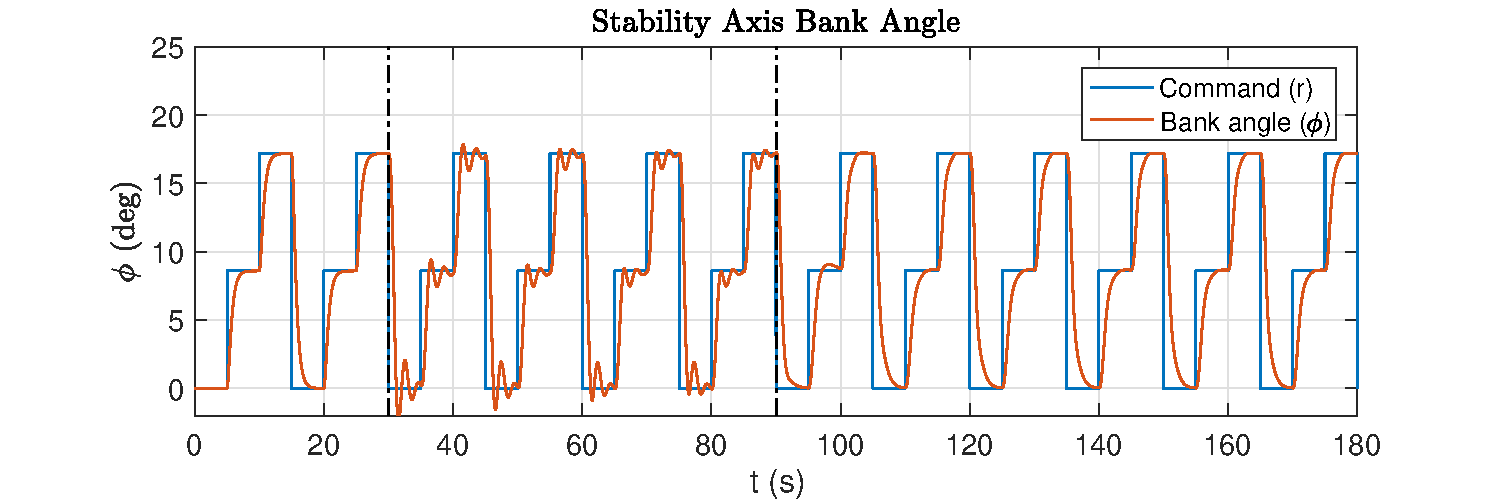
\includegraphics[width=\columnwidth]{phi_pole.pdf}
	\caption{Command ($r$) and output ($\phi$): under nominal operation ($t \leq 30$ s), after the change in actuator dynamics ($30$ s $< t \leq 90$ s), and after a corrective action to switch the controller ($t > 90$ s)}
	\label{fig:command_and_output}
\end{figure}

\begin{figure}[h!]
	\centering
	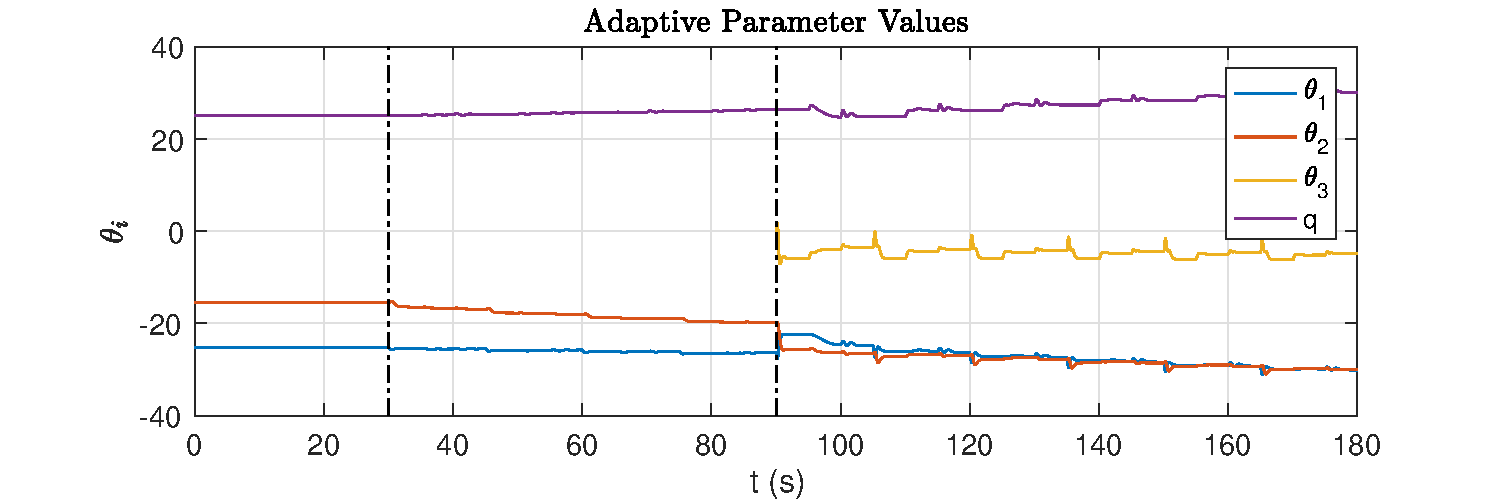
\includegraphics[width=\columnwidth]{theta_pole.pdf}
	\caption{Adaptive feedback gains for the same simulation example as in Figure \ref{fig:command_and_output}: under nominal operation ($t \leq 30$ s), after the change in actuator dynamics ($30$ s $< t \leq 90$ s), and after a corrective action to switch the controller ($t > 90$ s)}
	\label{fig:theta}
\end{figure}

\begin{figure}[h!]
	\centering
	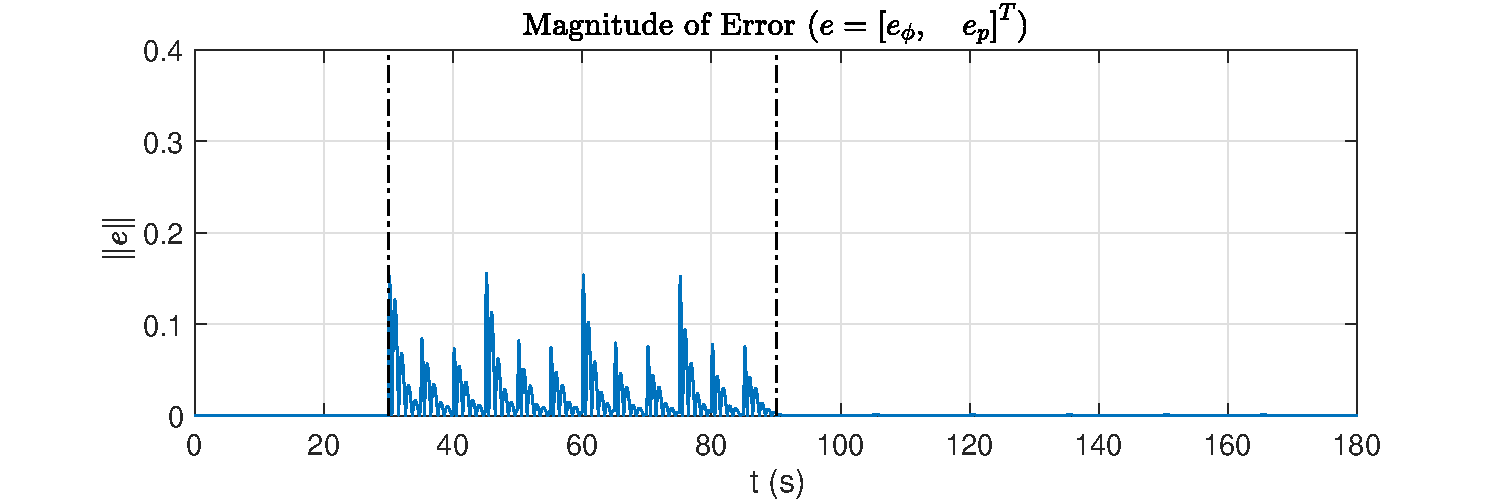
\includegraphics[width=\columnwidth]{e_pole.pdf}
	\caption{The tracking error $e$ for the same simulation example as in Figure \ref{fig:command_and_output}: under nominal operation ($t \leq 30$ s), after the change in actuator dynamics ($30$ s $< t \leq 90$ s), and after a corrective action to switch the controller ($t > 90$ s)}
	\label{fig:error}
\end{figure}

From Figures \ref{fig:command_and_output}, \ref{fig:theta}, and \ref{fig:error}, it is clear that after an initial adaptation period, the adaptive controller with third-order reference model dynamics converges on the desired feedback/feedforward gains, returning the roll control to its satisfactory performance without requiring any manual control from the human pilot. The action required from the human pilot is in the detection and diagnosis of the anomaly in dynamical behavior, leading to the addition of feedback on $\hat{\dot{p}}$ as a corrective action. 

Taking average parameter values over time $\Delta t$ at the end of each stage of simulation (Nominal, Post-Anomaly, Post-Correction)
\begin{align}
	\bar{\theta}_{t_i} &= \frac{1}{\Delta t} \int_{t_{f,i}-\Delta t}^{t_{f,i}} \theta(t) dt, \qquad i = [1, 2, 3] \label{eqn:theta_bar}\\
	\bar{q}_{t_i} &= \frac{1}{\Delta t} \int_{t_{f,i}-\Delta t}^{t_{f,i}} q(t) dt, \qquad i = [1, 2, 3] \label{eqn:q_bar}
\end{align}
with $\Delta t = 5$s, $t_f = [30, \quad 90, \quad 180]$ allows us to define a closed-loop frequency response which is representative of controller performance after parameter adaptation in each stage. Figure \ref{fig:step_pole} shows the closed-loop unit step input responses with $(\bar{\theta}_i, \bar{q}_i)$ for $i = [1, 2, 3]$ plotted alongside the ideal response during nominal operation, demonstrating how the characteristics of nominal operation are recovered with the adaptive controller with three feedback parameters.

\begin{figure}[h!]
	\centering
	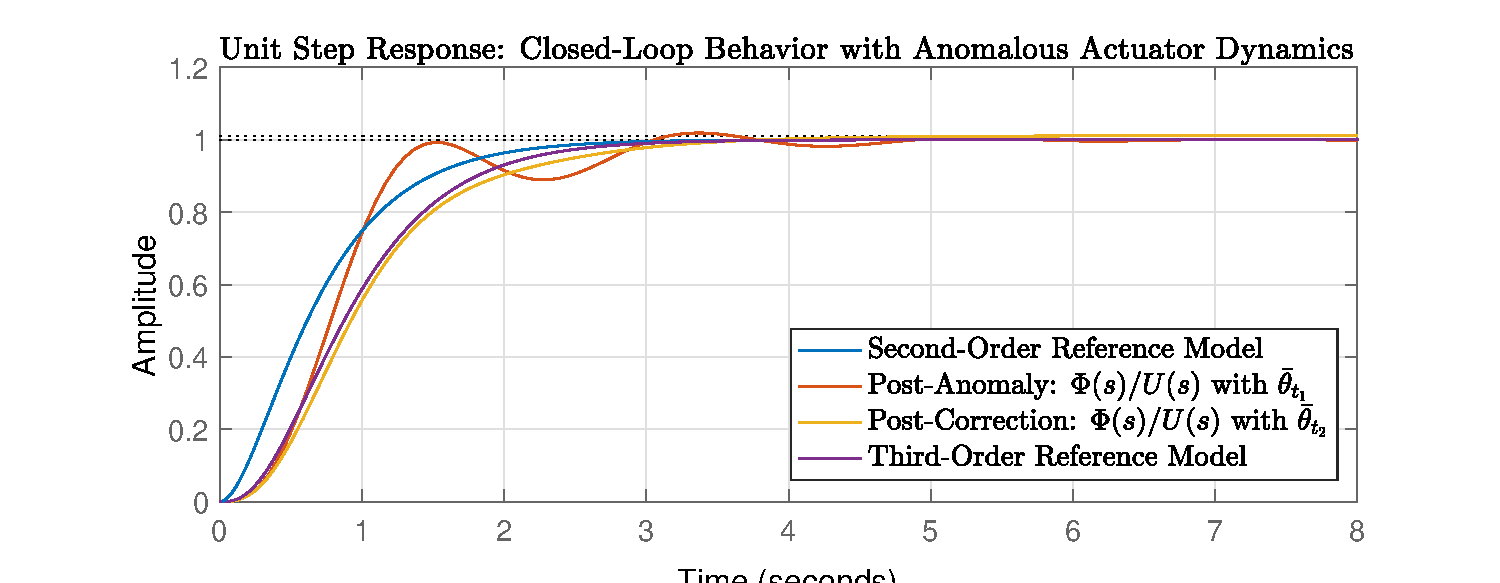
\includegraphics[width=\columnwidth]{step_pole.pdf}
	\caption{Unit step responses for closed-loop transfer functions at different stages of simulation in case (i), demonstrating performance improvement after corrective action}
	\label{fig:step_pole}
\end{figure}

\subsection{Time-Delayed Sensor Measurements}
A time delay of $\tau = 0.200$s is added to the plant (\ref{eqn:2nd_order_lateral}) between the state measurements and their use in control input computation. The reference models given by (\ref{eqn:rm_2}) and 
\begin{equation}
	\dot{x}_m' = \underbrace{\begin{bmatrix}
		\hfil 0 & \hfil 1 & \hfil 0\\ \hfil 0 & \hfil 0 & \hfil 1 \\ -32 & -32 & -10
	\end{bmatrix}}_{A_m'} x_m' + \underbrace{\begin{bmatrix}
		0 \\ 0 \\ 32
	\end{bmatrix}}_{B_m'} r - \underbrace{\begin{bmatrix}
		-10 & -1 & \hfil 0 \\ \hfil 0 & \hfil -10 & \hfil -1 \\ \hfil 32 & \hfil 32 & \hfil 9.9
	\end{bmatrix}}_{L_m'} e'
	\label{eqn:rm_3_delay}
\end{equation}
\noindent are used in the Nominal and Post-Correction intervals, respectively. With $\Phi_\sigma(s)$ defined as the delayed bank angle measurement, the change in the transfer function $\Phi_\sigma(s)/U(s)$ is thus
\begin{equation}
		\frac{\Phi_\sigma(s)}{U(s)} = \begin{cases}
			\frac{0.318}{s^2 + 1.10s} & t < t_{s,p}\\
			\frac{0.318}{s^2 + 1.10s}e^{-0.20 s} & t \geq t_{s,p}
		\end{cases} 
\end{equation}

% TODO put this in diff eq form
Using the first-order delay approximation (\ref{eqn:delay_approx_diffeq}), so that $e^{-0.20 s}$ is approximated as $1/(1+0.20s)$, the feedback and feedforward gains which would give the desired closed-loop response for $\Phi_\sigma(s)/U(s)$ are
\begin{align}
	\theta^*(t) = & \begin{cases} \begin{bmatrix} -25.16, & -15.41 \end{bmatrix} & t < t_{s,p} \\ \begin{bmatrix}-20.13, & -16.67, & -2.45\end{bmatrix} & t \geq t_{s,p} \end{cases} \\
	q^*(t) = &\begin{cases} 25.16 & t < t_{s,p} \\ 20.13 & t \geq t_{s,p} \end{cases}
\end{align}

\noindent The learning rates chosen for this simulation were
\begin{align}
	\Gamma_\theta  = & \begin{cases}
		10 I_2 & t < t_{s,c}\\
		\text{diag}(10.0, 10.0, 0.1) & t \geq t_{s,c}
 	\end{cases} \\
	\gamma_q  = &\quad 10.0 \qquad ~ \qquad ~ \qquad ~ \quad \forall t
\end{align}

\noindent where the learning rate on $\hat{\dot{p}}$ is lower than that used in the simulation of case (i). This lower learning rate was needed as the approximation of the time delay as a first-order lag is fairly restrictive. In addition, a projection operator with the following constant parameters (\ref{eqn:proj_function}) was used to limit $\dot{\theta}(t)$
\begin{align}
	\varphi_m = & \begin{bmatrix}
		300, & 200, & 25
	\end{bmatrix} \\
	\varphi_{\epsilon} = & \begin{bmatrix}
		50, & 50, & 25
	\end{bmatrix}\end{align}
\noindent and the following constant parameters for the projection operator limiting $\dot{q}(t)$
\begin{align}
	\varphi_m = &~ 300\\
	\varphi_{\epsilon} = &~ 50
\end{align}

\begin{figure}[h!]
	\centering
	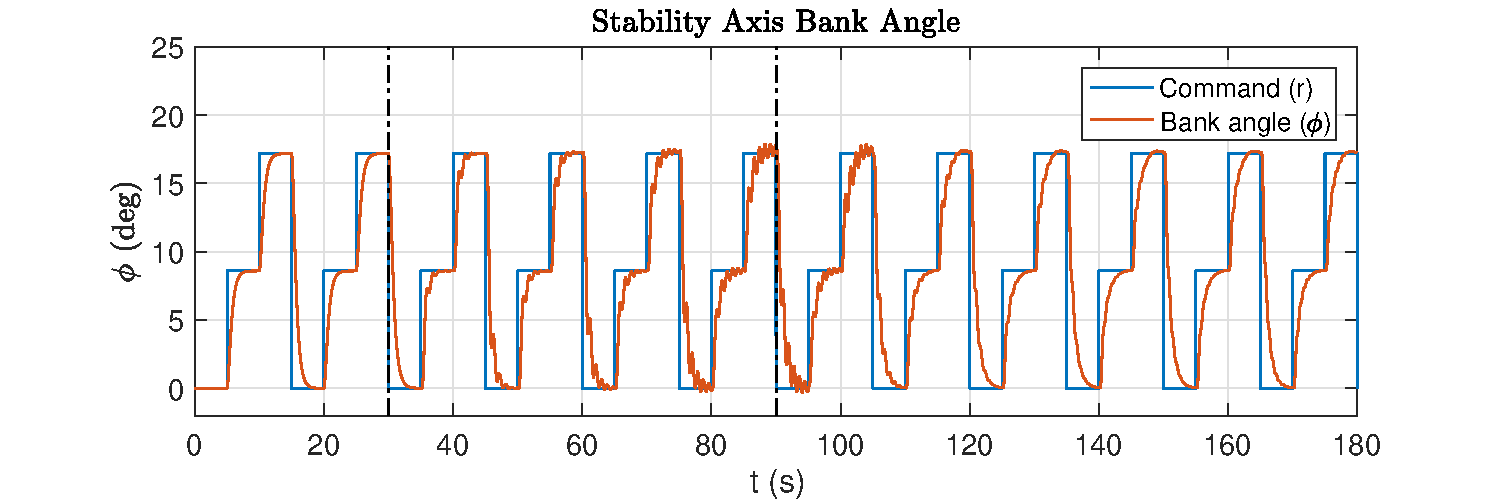
\includegraphics[width=\columnwidth]{phi_delay.pdf}
	\caption{Command ($r$) and output ($\phi$): under nominal operation ($t \leq 30$ s), after the sudden addition of a time delay ($30$ s $< t \leq 90$ s), and after a corrective action to switch the controller ($t > 90$ s)}
	\label{fig:command_and_output_d}
\end{figure}

\begin{figure}[h!]
	\centering
	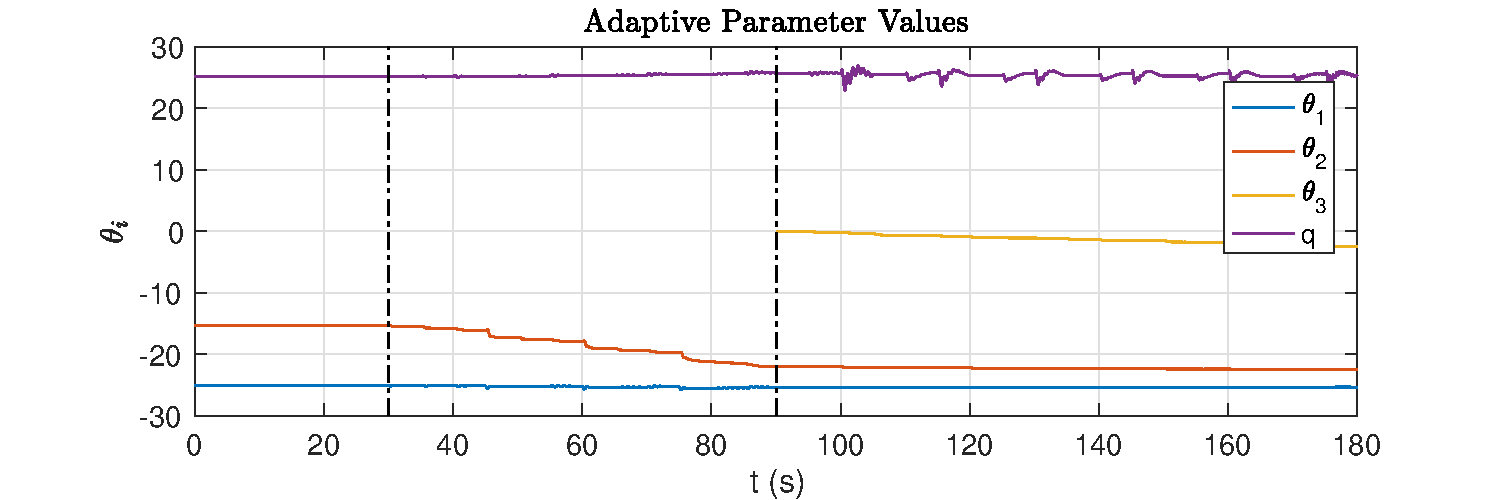
\includegraphics[width=\columnwidth]{theta_delay.pdf}
	\caption{Adaptive feedback gains for the same simulation example as in Figure \ref{fig:command_and_output_d}: under nominal operation ($t \leq 30$ s), after the sudden addition of a time delay ($30$ s $< t \leq 90$ s), and after a corrective action to switch the controller ($t > 90$ s)}
	\label{fig:theta_d}
\end{figure}

\begin{figure}[h!]
	\centering
	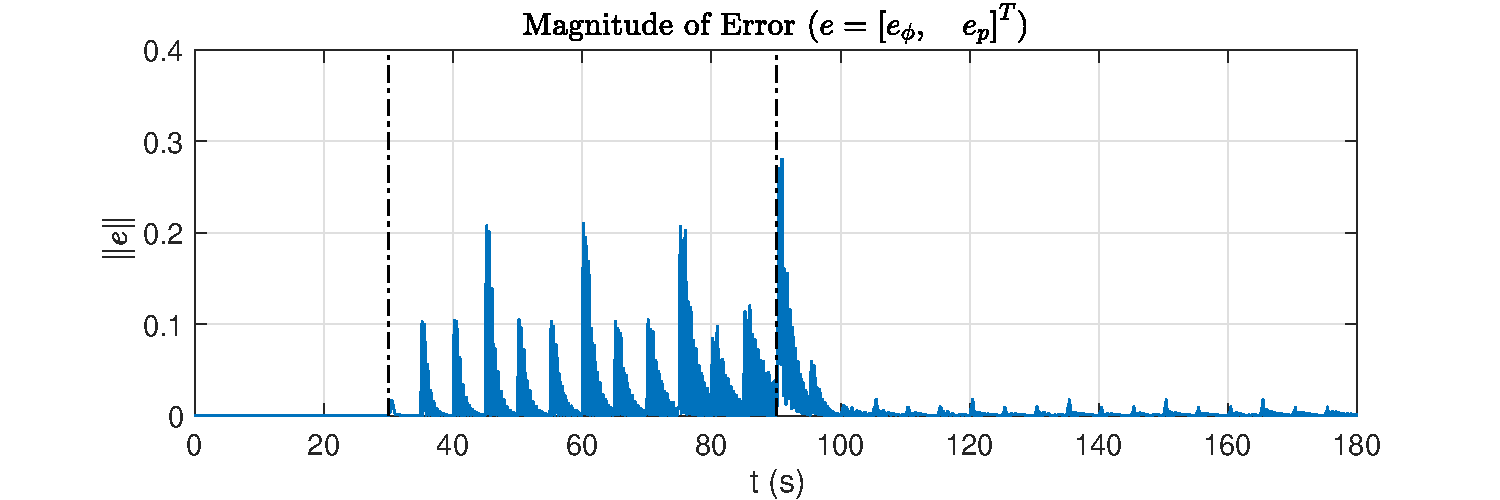
\includegraphics[width=\columnwidth]{e_delay.pdf}
	\caption{The tracking error $e$ for the same simulation example as in Figure \ref{fig:command_and_output_d}: under nominal operation ($t \leq 30$ s), after the sudden addition of a time delay ($30$ s $< t \leq 90$ s), and after a corrective action to switch the controller ($t > 90$ s)}
	\label{fig:error_d}
\end{figure}

The resulting responses of the shared controller are shown in Figures \ref{fig:command_and_output_d}, \ref{fig:theta_d}, and \ref{fig:error_d}. From these results, we see that the MRAC controller with two feedback parameters has trouble tracking the commanded bank angle after the introduction of an anomaly, but the addition of a third feedback parameter ($\hat{\dot{p}}$) and a corresponding increase in the dimension of the reference model allows the controller to recover a reasonable tracking performance. It is worth noting that the model-following error does not converge to zero even with the MRAC controller given by (\ref{eqn:control_law}), (\ref{eqn:thetadot_projection}), (\ref{eqn:qdot_projection}), and (\ref{eqn:rm_3}), because of the time delay approximation. 

The transfer functions used to generate step response plots in Figure \ref{fig:step_delay} use (\ref{eqn:theta_bar}) and (\ref{eqn:q_bar}) for average parameter values. Although the step response characteristics of Post-Correction differ more from nominal operation compared to case (i), the closed-loop response of Post-Correction is significantly more satisfactory than Post-Anomaly.

\begin{figure}[h!]
	\centering
	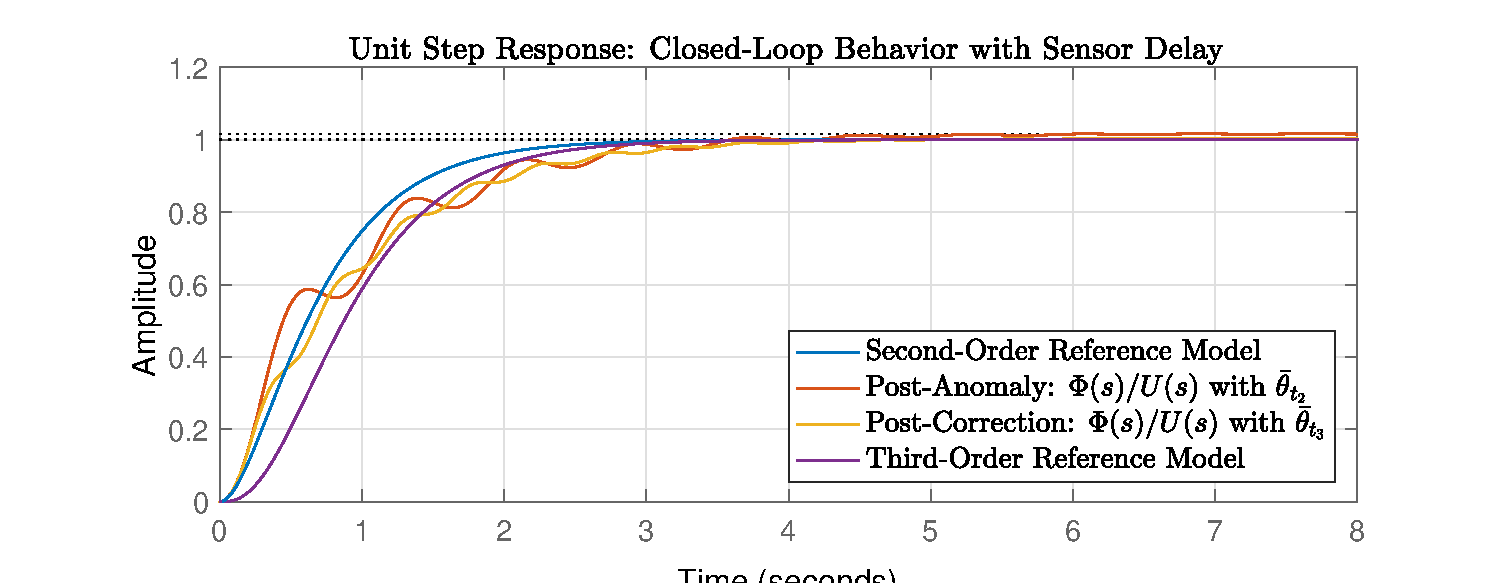
\includegraphics[width=\columnwidth]{step_delay.pdf}
	\caption{Unit step responses for closed-loop transfer functions at different stages of simulation in case (ii), demonstrating performance improvement after corrective action}
	\label{fig:step_delay}
\end{figure}

The shared control solution introduced in Chapter \ref{sec:shared_ctrl} is applied to the problem introduced in Section \ref{sec:mimo_problem} on a high altitude, long endurance (HALE) very flexible aircraft (VFA) model. The aircraft model used in simulation, developed by \cite{gibson2011modeling} for longitudinal control design applications, is rendered in Figure \ref{fig:vfa} and described in Section \ref{subsec:vfa_model}. The results of numerical simulations on the control and anomaly recovery with this MIMO plant are then presented in Section \ref{subsec:sims}, comparing the shared anomaly response to alternative anomaly responses.

\section{Output Feedback}

\subsection{HALE Aircraft Model}\label{subsec:vfa_model}
%HALE VFA.
High altitude long endurance (HALE) aerial platforms, such as the solar-electric NASA/AeroVironment Helios and Facebook Aquila, have unique design considerations to satisfy goals of uninterrupted weeks- or months-long operation. To reduce power draw, HALE aircraft designs save mass by allowing wings to bend, and may be classified as very flexible aircraft (VFA). Compared to typical fixed-wing aircraft, these aircraft operate at low speed, and may use low-bandwidth actuators which must be accounted for in control design. HALE VFA platforms are likely to have significant modeling uncertainties and online variation in dynamics due to flexible effects and degradation over long-term operation. Although these platforms are unmanned aerial vehicles (UAVs), they require supervision from remote human operators.

\begin{figure}[htbp]
	\centering
	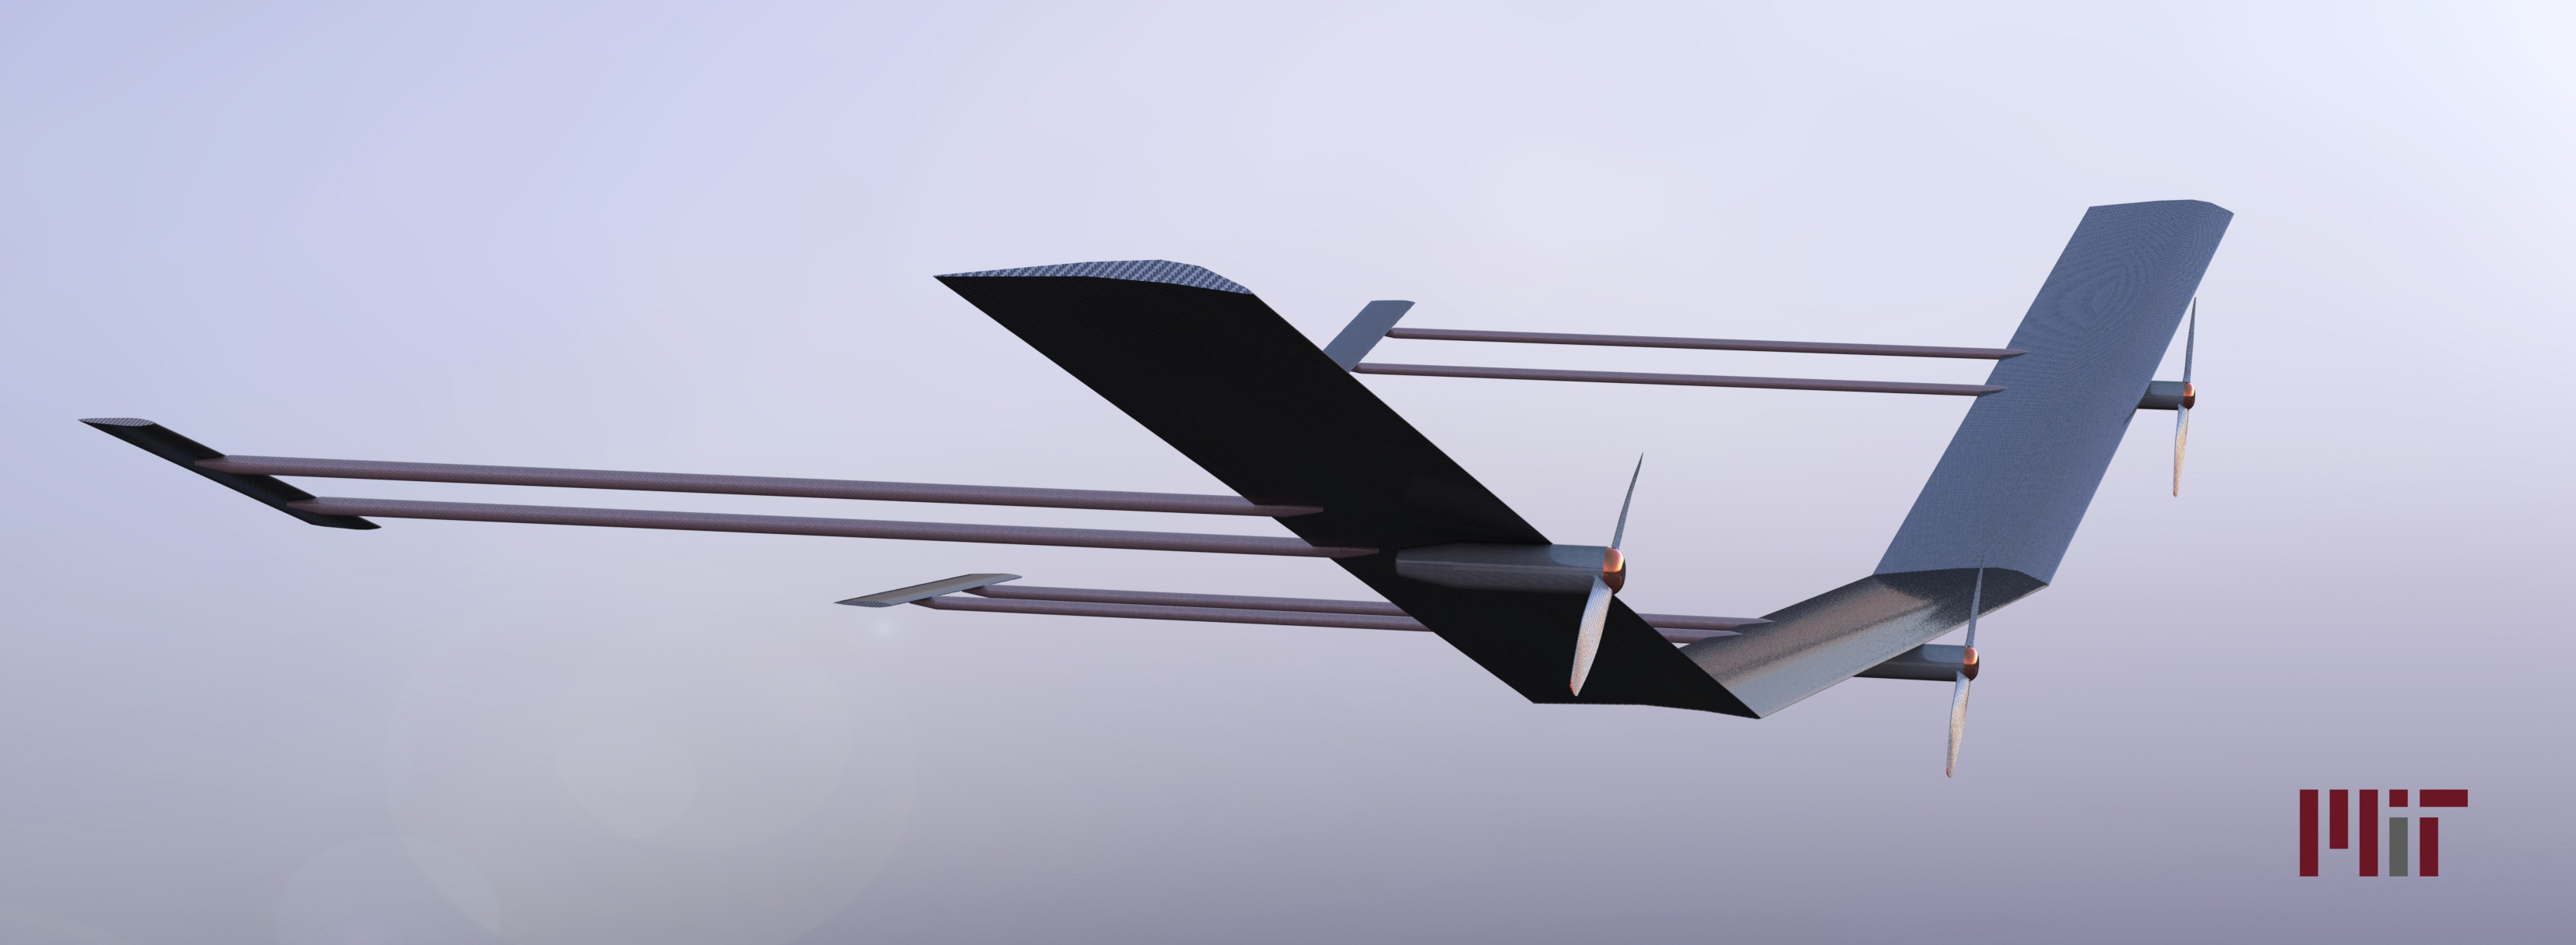
\includegraphics[width=0.95\columnwidth]{VFA_16.jpg}
	\caption{Rendering of very flexible aircraft model}
	\label{fig:vfa}
\end{figure}

The aircraft model used in simulation represents the nonlinear longitudinal dynamics of a HALE VFA concept with three rigid lifting sections, hinged together such that the aircraft is able to bend at the joints of the three sections. The pitch mode dynamics of this nonlinear model is defined by the state vector
\begin{equation}
x_{\text{vfa}} = \begin{bmatrix}
~V~\\
\alpha \\
h \\
\theta \\
q\\
\eta\\
\dot{\eta}
\end{bmatrix} =
\begin{bmatrix}
	 $Airspeed (ft/s)$\\ $Angle of attack (rad)$\\ $Altitude (ft)$\\ $Pitch angle (rad)$\\ $Pitch rate (rad/s)$\\ $Dihedral (rad)$\\ $Dihedral rate (rad/s)$
\end{bmatrix}
\end{equation}

We linearize and trim the aircraft in straight and level flight using the inputs
\begin{equation}
	u_{\text{vfa}} = \begin{bmatrix}
\delta_{th} \\
\delta_{a,c} \\
\delta_{a,o} \\
\delta_{e,c} \\
\delta_{e,o} 
\end{bmatrix} = \begin{bmatrix}
		$Thrust (lbf)$\\
		$Center aileron (rad)$\\
		$Outer aileron (rad)$\\
		$Center elevator (rad)$\\
		$Outer elevator (rad)$
	\end{bmatrix}
\end{equation}

Assuming small deviations in altitude, the state vector corresponding to (\ref{eq:plant_dynamics}) is
\begin{equation}
	x_p = \begin{bmatrix}
V & \; \alpha & \; \theta & \; q & \; \eta & \; \dot{\eta}
\end{bmatrix}^T.
\end{equation}

We consider the control task of tracking commands for the dihedral angle and vertical acceleration, using control inputs $\delta_{a,o}$ and $\delta_{e,c}$ only, so the vector $u_p$ in (\ref{eq:plant_dynamics}) is
\begin{equation}
	u_p = \begin{bmatrix}
\delta_{a,o} & \; \delta_{e,c}
\end{bmatrix}^T.
\end{equation}

Regulation of the dihedral angle is desired, as a large dihedral angle is inefficient for lift generation and introduces instability in the open-loop dynamics, while a small dihedral angle will require more control effort to hold, increasing drag and power requirements and imparting twisting moments on the aircraft. 

The measurements available for control design are the pitch rate, dihedral angle, and vertical acceleration, leading to plant outputs
\begin{equation}
\begin{aligned}
y_p =& \, \Big[\; q \; \Big] \;= \Big[\: \text{Pitch rate (rad/s)} \:\Big] \\
z_p =& \begin{bmatrix}
\eta \\
A_z
\end{bmatrix} =\begin{bmatrix}
	$Dihedral angle (rad)$\\
	$Vertical acceleration (ft/s)$
\end{bmatrix}		
\end{aligned}
\end{equation}
and the outputs for the augmented plant (\ref{eq:augmented_plant}),
\begin{equation}
y = \begin{bmatrix}
	q \\ \int{z_p - z_{cmd}}
\end{bmatrix}, \quad z = z_p.
\end{equation}

For numerical simulations, the VFA model is trimmed at an airspeed of $68$ ft/s, altitude of $40,000$ ft, $2.8^\circ$ angle of attack and pitch angle (level flight), and dihedral angles ranging from $0$ to $20^\circ$ in $1^\circ$ increments. Figure \ref{fig:trim-poles} shows pole locations of the linearized plant for different dihedral angles, and Figure \ref{fig:trim-poles-zoom} shows instability of the linearized plant when trimmed above $11^\circ$ dihedral. Figure \ref{fig:trim-inputs} shows the thrust and control surface deflections for the trimmed VFA model over a range of dihedral angles.

\begin{figure}[htbp]
	\centering
	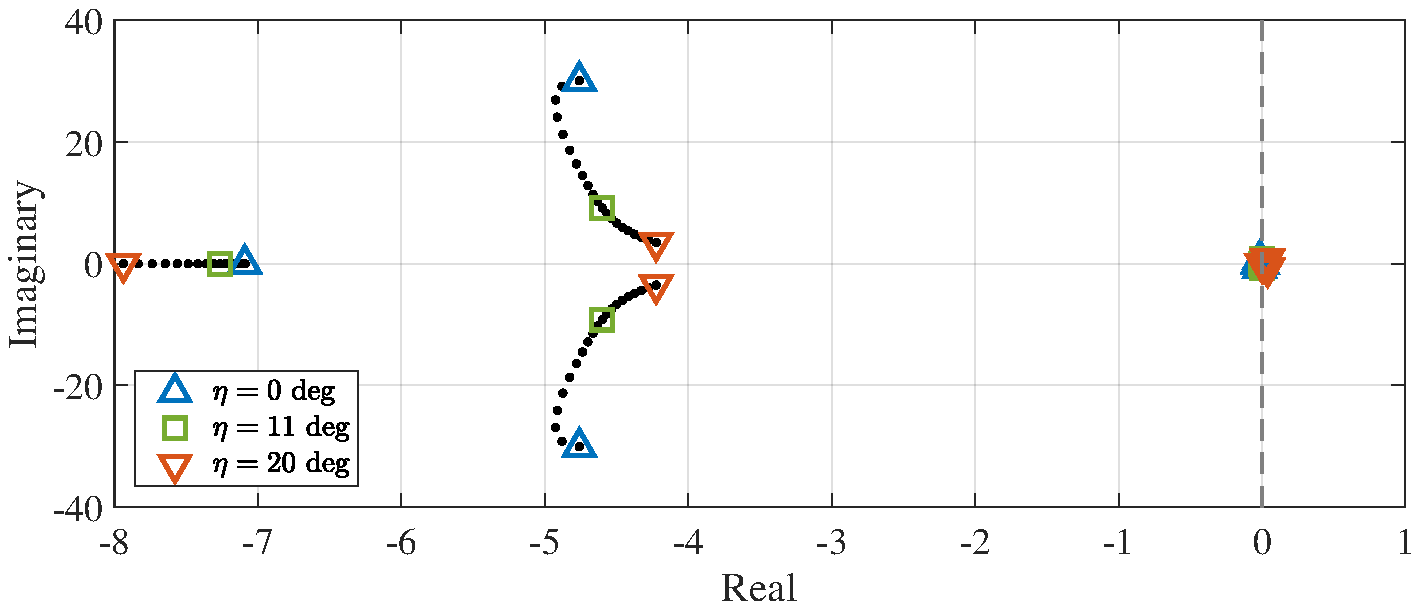
\includegraphics[width=0.95\columnwidth]{trim-poles-2.pdf}
	\caption{Poles of linearized system for different dihedral angles}
	\label{fig:trim-poles}
\end{figure}

\begin{figure}[htbp]
	\centering
	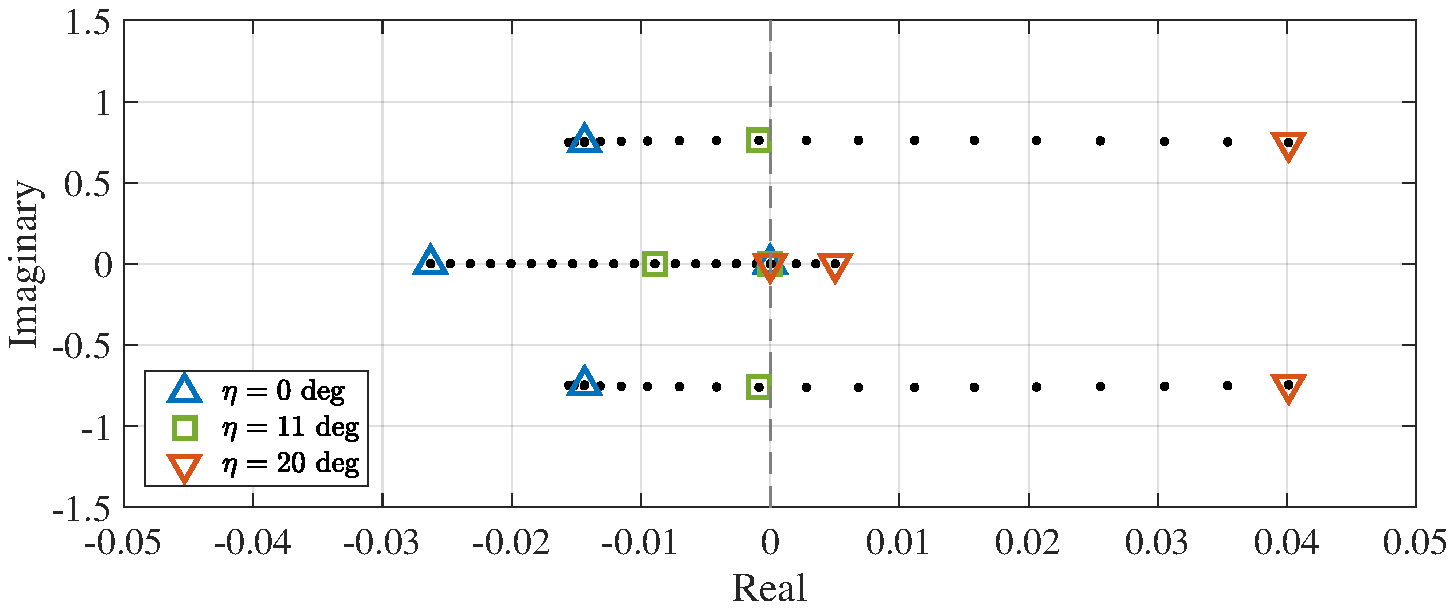
\includegraphics[width=0.95\columnwidth]{trim-poles-zoom-2.pdf}
	\caption{Dominant poles of linearized system, which move into the right-half complex plane when $\eta > 11^\circ$}
	\label{fig:trim-poles-zoom}
\end{figure}

\begin{figure}[htbp]
	\centering
	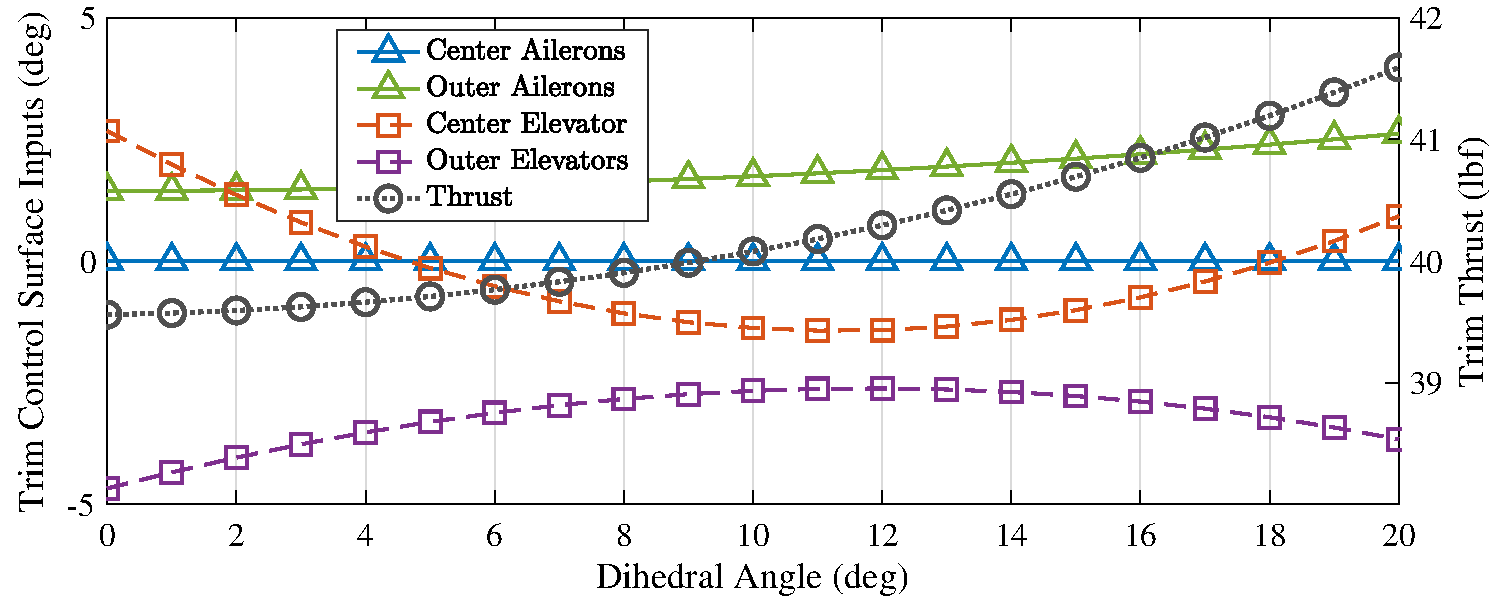
\includegraphics[width=0.95\columnwidth]{trim-inputs-3.pdf}
	\caption{Actuator trim at different dihedral angles}
	\label{fig:trim-inputs}
\end{figure}

The plant is augmented with a linear actuator model corresponding to (\ref{eq:first_order_act}) in the nominal case and (\ref{eq:second_order_act}) in the presence of anomalous dynamics. The vehicle simulation with first-order actuators (\ref{eq:first_order_act}) uses time constants $(\hat{\tau},\;\tau) = (0.5,\,2)$s in the control model and the actual plant, respectively, corresponding to
\begin{equation}
D_1 = 2 I_2, \quad \Theta_1 = -1.5 I_2
\end{equation}
where $\Theta_1$ is unknown for control design, and $I_2$ is the $2 \times 2$ identity matrix. 

Simulation of the anomalous dynamics (\ref{eq:second_order_act}) uses second-order actuators with cutoff frequencies $(\hat{\omega}_c,\; \omega_c) = (2 ,\; 1)$ rad/s and damping ratios $(\hat{\zeta},\; \zeta) = (0.7,\; 0.8)$ in the control model and actual plant, respectively, corresponding to
\begin{equation}
\begin{bmatrix}
	D_1 \\ D_2
\end{bmatrix} = \begin{bmatrix}
	4 I_2 \\ 2.8 I_2
\end{bmatrix}, \quad \begin{bmatrix}
	\Theta_1 \\ \Theta_2 
\end{bmatrix} = \begin{bmatrix}
	-3.75 I_2 \\ -2 I_2
\end{bmatrix}
\end{equation}
where $\Theta_1$ and $\Theta_2$ are unknown for control design. The uncertainty matrices $\Theta_p$ and $\Lambda$ are given by
\begin{equation}
\begin{gathered}
\Theta_{p}^{T}=\begin{bmatrix}
0.6 & -4.52 & \; 0 & \hfill 0.05 & \hfill 0.41 & \hfill 1.47\\
0.1 & \hfill 1.83 & \; 0 & -0.02 & -0.35 & -0.59
\end{bmatrix}\\ \Lambda = 0.2 I_2 \end{gathered}
\end{equation}
representing a poor linearization of the nonlinear model, and an 80\% reduction in actuator effectiveness.

\subsection{Numerical Simulations and Results} \label{subsec:sims}
We begin by simulating the HALE VFA under nominal autonomous control, responding to step inputs in commands for the dihedral angle and vertical acceleration, with the following three variants.
\begin{description}
	\item[Nom-1] Baseline RSLQR without uncertainty in control model
	\item[Nom-2] Baseline RSLQR with uncertainty in control model ($\Theta_p$, $\Lambda_p$, and $\Theta_1$)
	\item[Nom-3] Baseline RSLQR + MRAC with uncertainty in control model ($\Theta_p$, $\Lambda_p$, and $\Theta_1$)
\end{description}

\begin{figure}[htbp]
	\centering
	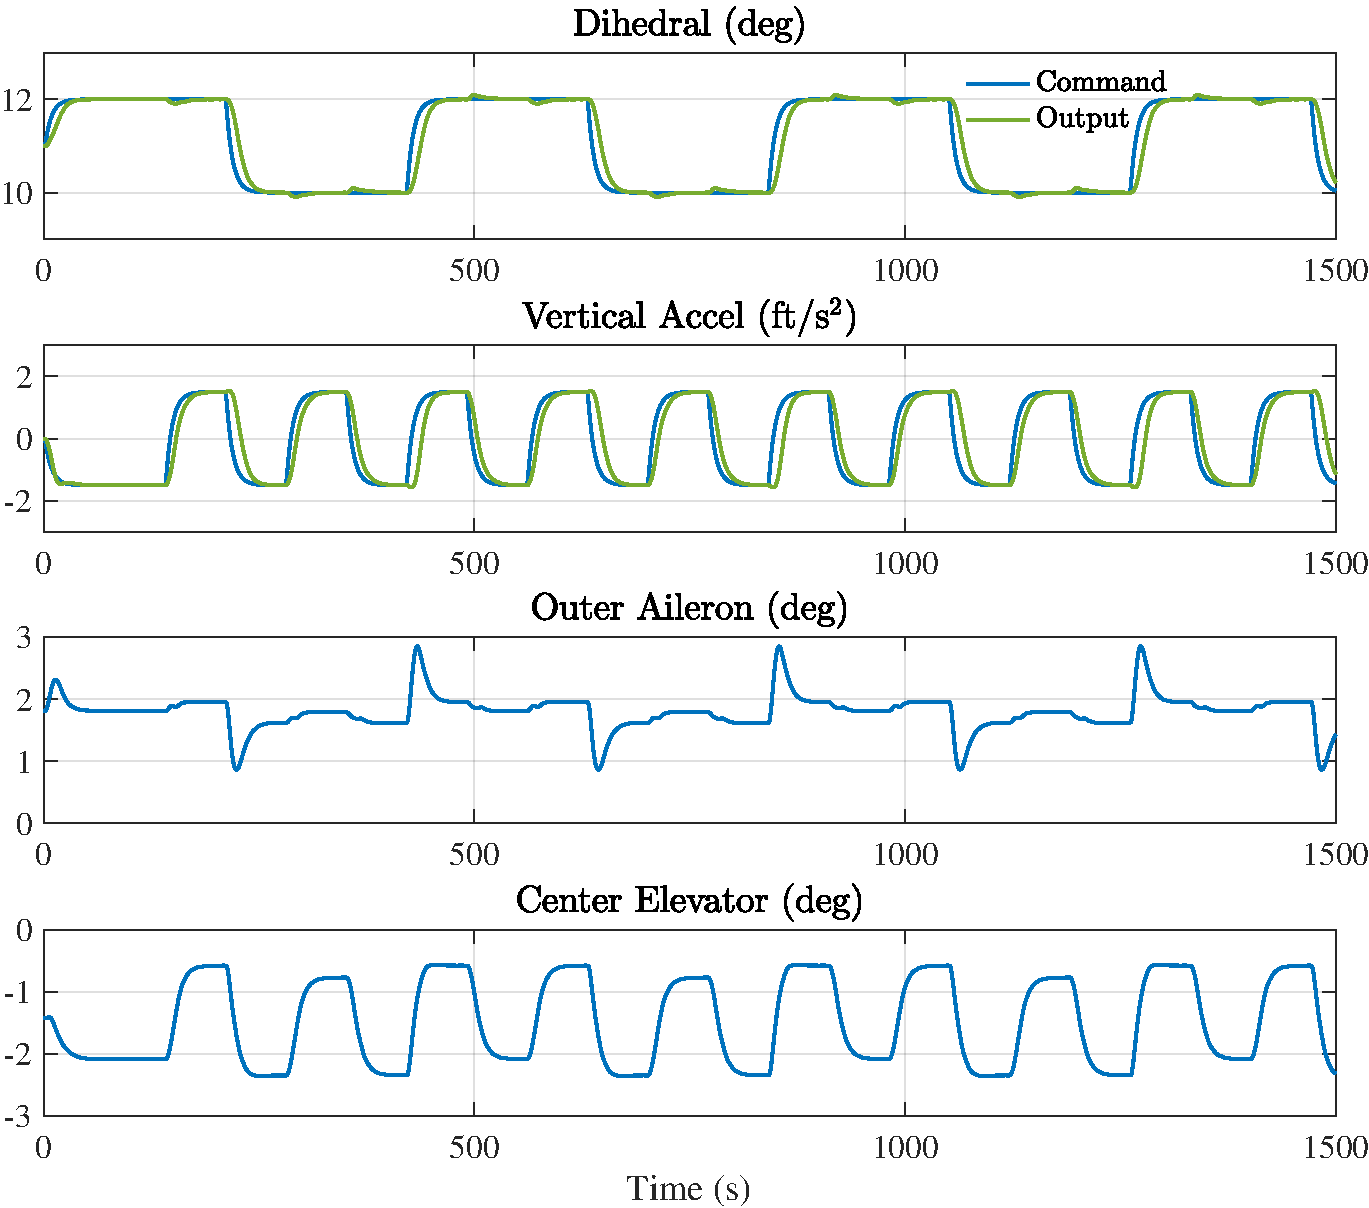
\includegraphics[width=\columnwidth]{nom1.pdf}
	\caption{Nom-1 simulation: RSLQR with no uncertainty in the control model}
	\label{fig:nom1}
\end{figure}

\begin{figure}[htbp]
	\centering
	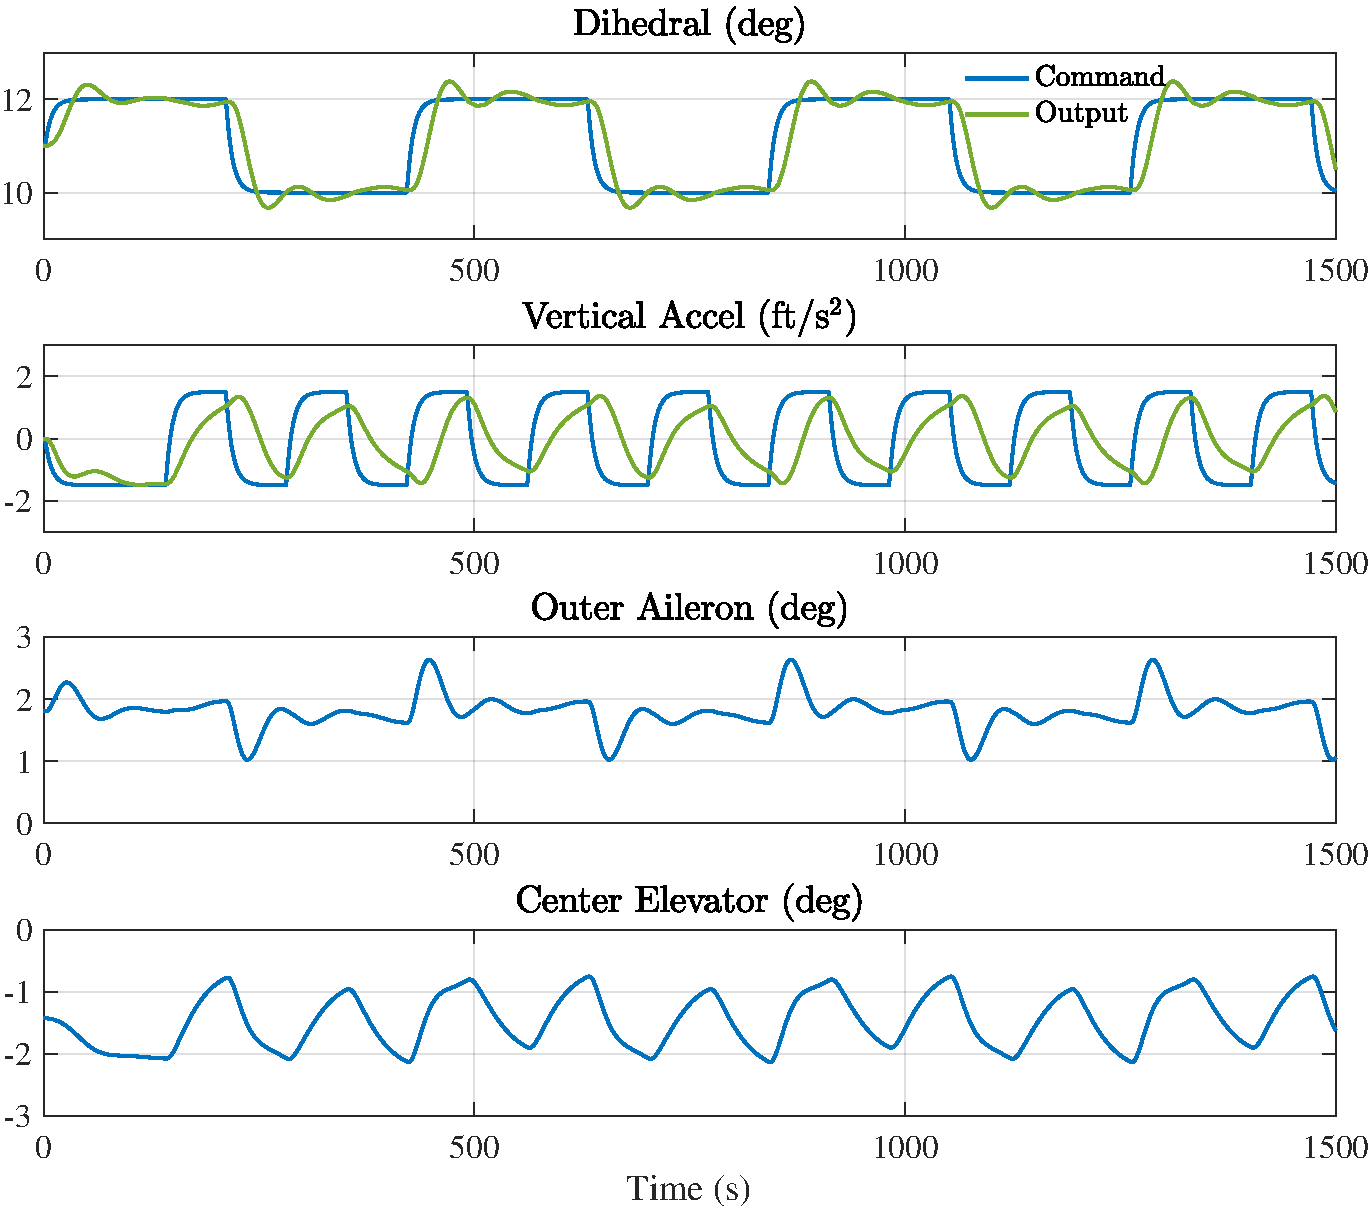
\includegraphics[width=\columnwidth]{nom2.pdf}
	\caption{Nom-2 simulation: RSLQR with uncertainties $\Theta_p$, $\Lambda_p$, and $\Theta_1$}
	\label{fig:nom2}
\end{figure}

\begin{figure}[htbp]
	\centering
	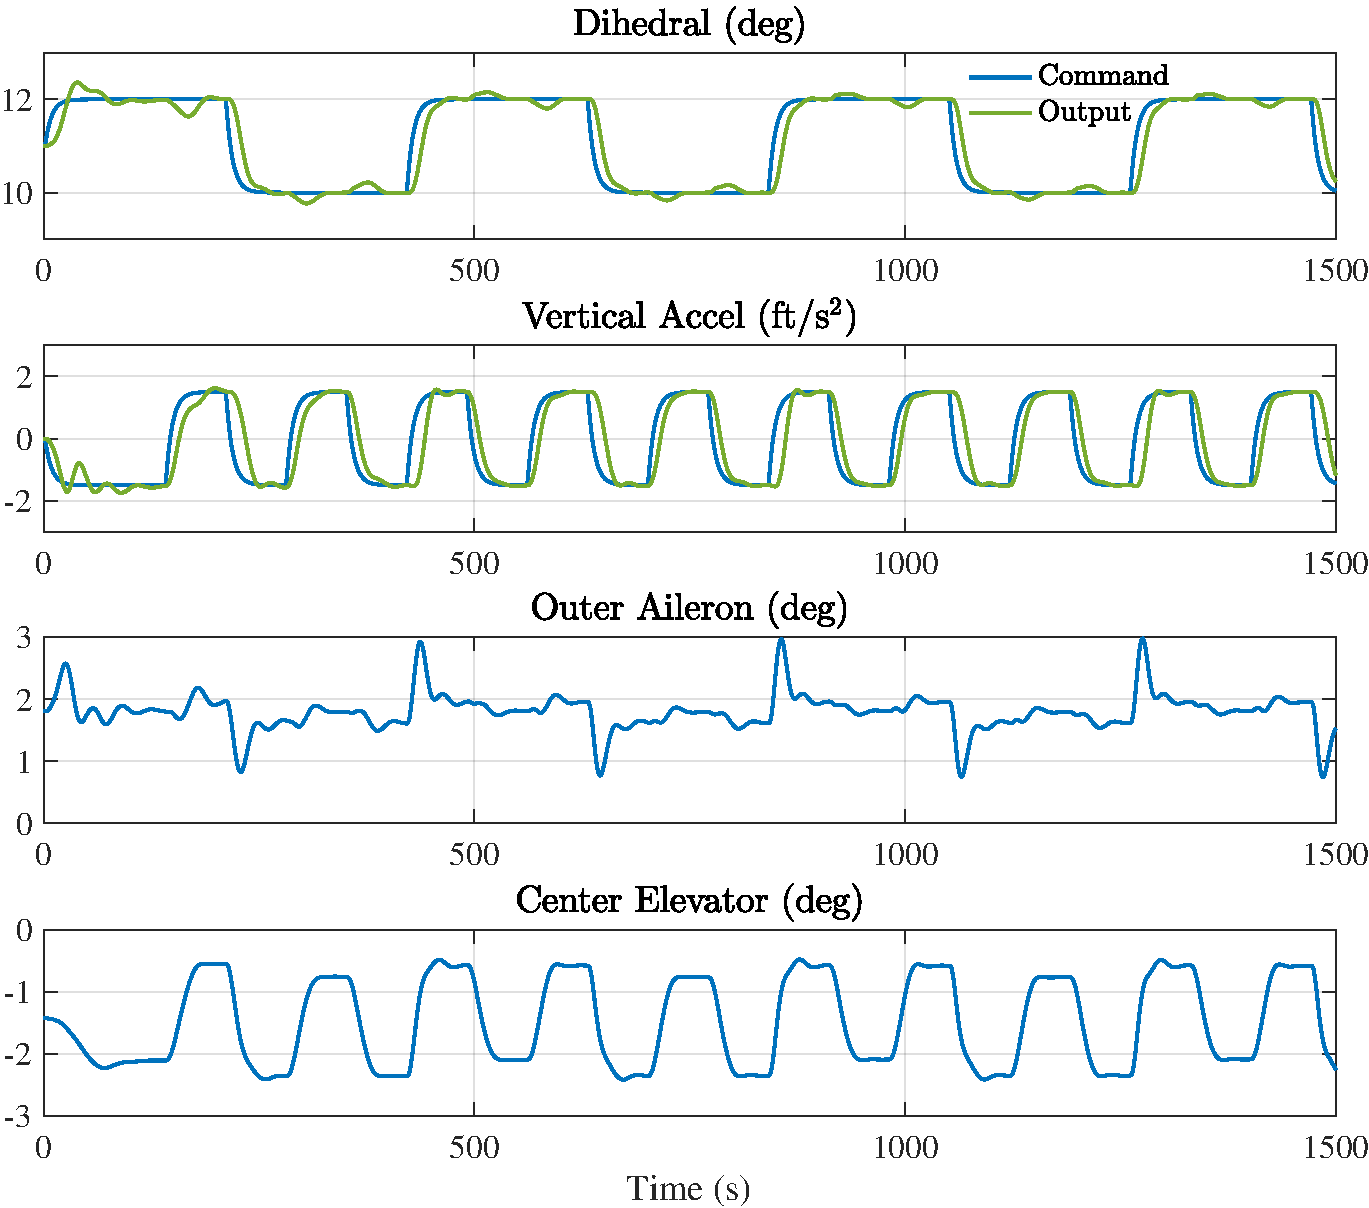
\includegraphics[width=\columnwidth]{nom3.pdf}
	\caption{Nom-3 simulation: RSLQR + MRAC with uncertainties $\Theta_p$, $\Lambda_p$, and $\Theta_1$}
	\label{fig:nom3}
\end{figure}

These simulations, presented in Figs. \ref{fig:nom1}, \ref{fig:nom2}, and \ref{fig:nom3} respectively, show how the MRAC controller with output feedback described in (\ref{eq:rd2-b1a})--(\ref{eq:rd2-adaptation}) is able to recover the desired closed-loop performance with uncertainty in plant and actuator parameters. With the baseline RSLQR controller only, the system suffers degraded command tracking performance in the presence of uncertainty (Fig. \ref{fig:nom2}), especially for vertical acceleration tracking.

We now simulate the introduction of a severe anomaly into the dynamics, causing the actuator dynamics to change suddenly from the uncertain first-order dynamics (\ref{eq:first_order_act}) to the uncertain second-order dynamics (\ref{eq:second_order_act}). The three responses to this anomaly which we will consider are
\begin{description}
	\item[AR-1 (Passive)] The RSLQR+MRAC autopilot retains control without intervention from the remote human supervisor
	\item[AR-2 (Manual)] The human operator takes over manual control of the affected vehicle
	\item[AR-3 (Shared)] Responsibilities are shared between the human pilot and autopilot as described in Section \ref{sec:shared_ctrl}
\end{description}

In these simulations, the vehicle operates in nominal operation with the RSLQR+MRAC control design for $0 \leq t < 600 s$. At $t = 600 s$, the vehicle's actuators change from first-order (\ref{eq:first_order_act}) to second-order (\ref{eq:second_order_act}). Figs. \ref{fig:ar1}--\ref{fig:ar1-err} show the result of a passive response (AR-1) in which the human operator ignores vehicle performance degradation and allows the adaptive controller to continue operating on the plant with severely anomalous dynamics. The closed-loop system loses stability, leading to oscillations in vehicle output and eventual structural failure of the VFA at $t = 960s$, 6 minutes after the introduction of second-order actuator dynamics. It is worth noting the rapid increase in magnitude of the adaptive parameters and the magnitudes of both tracking and measurement output error signals after the introduction of anomalous dynamics. For comparison to a baseline without adaptive control, a passive response using only the RSLQR controller leads to structural failure following the anomaly, at $t = 1240s$.

\begin{figure}[htbp]
	\centering
	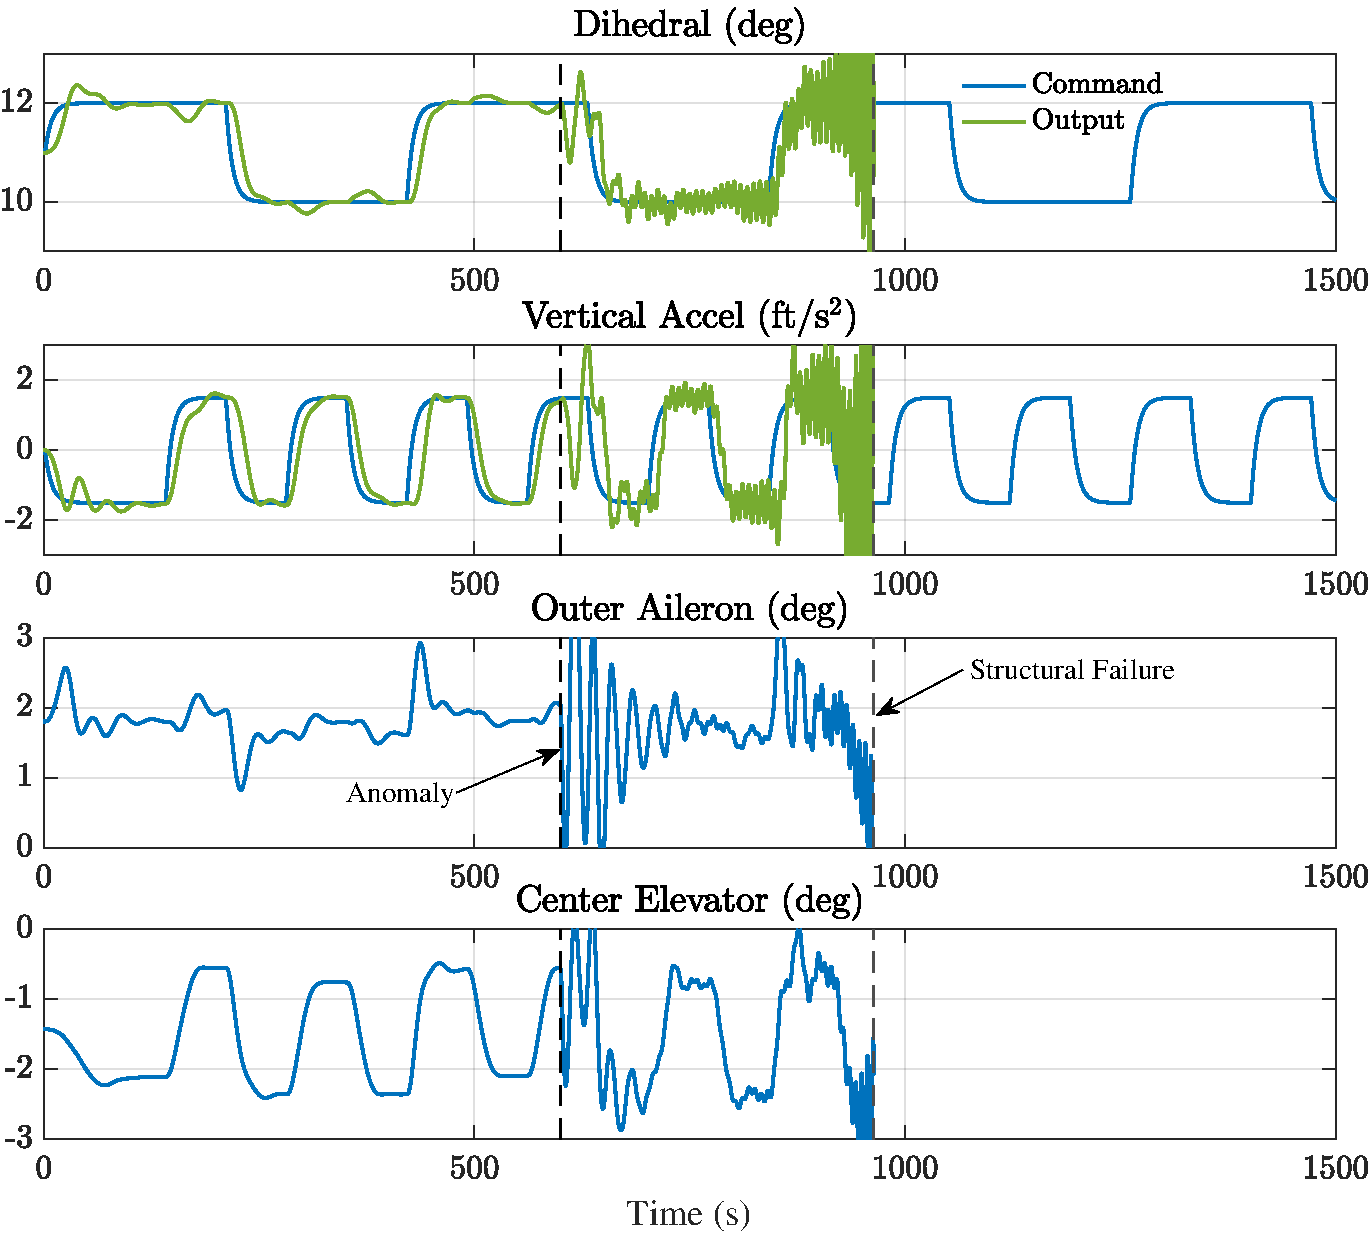
\includegraphics[width=\columnwidth]{ar1.pdf}
	\caption{AR-1 simulation: passive response to dynamical anomaly results in structural failure after 6 minutes}
	\label{fig:ar1}
\end{figure}

\begin{figure}[htbp]
	\centering
	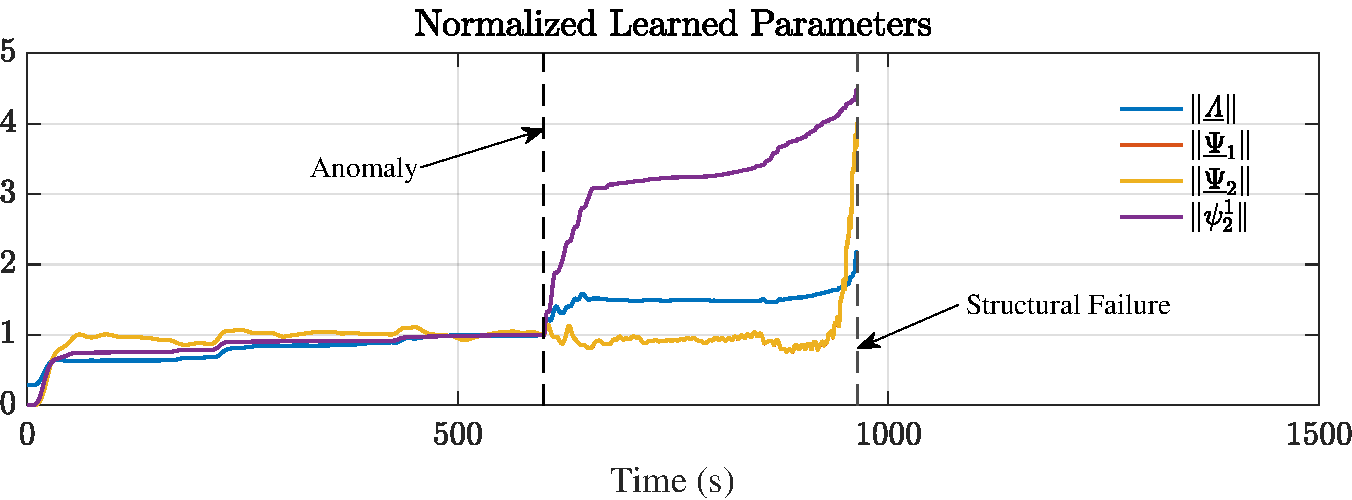
\includegraphics[width=\columnwidth]{ar1-params.pdf}
	\caption{AR-1 simulation: adaptive parameters diverge as controller struggles to adapt to unmodeled dynamics}
	\label{fig:ar1-params}
\end{figure}

\begin{figure}[htbp]
	\centering
	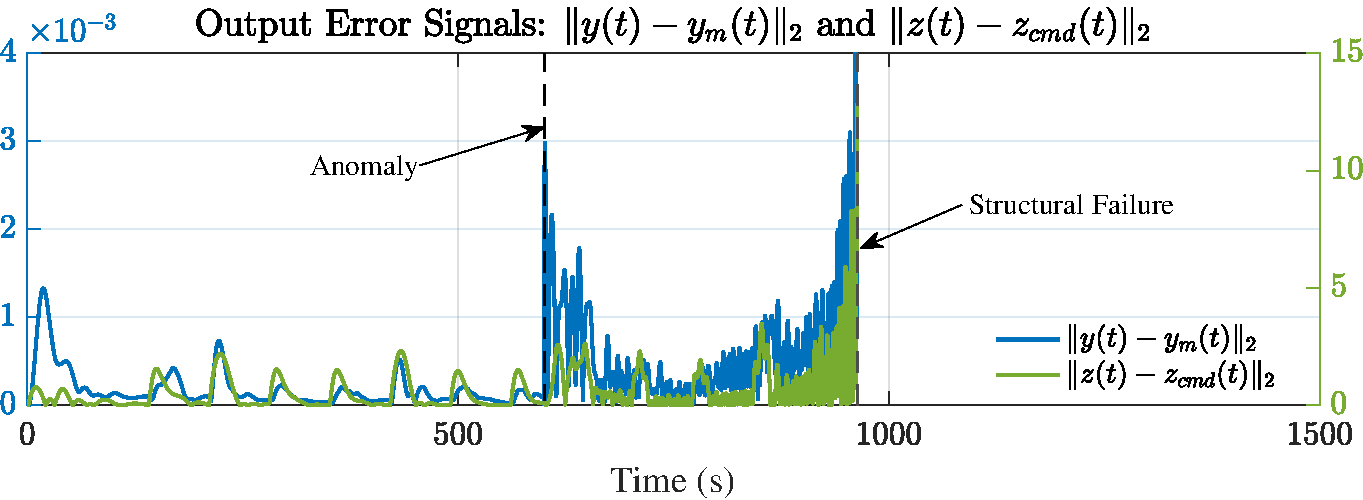
\includegraphics[width=\columnwidth]{ar1-err.pdf}
	\caption{AR-1 simulation: model-following output error and command tracking error grow due to anomalous dynamics}
	\label{fig:ar1-err}
\end{figure}

Numerical simulations of the AR-2 response (purely manual control) are not carried out, as they are not deterministic and require high-fidelity \textit{human-in-the-loop} experiments to characterize. The limitations of such a response -- in which the human operator's role changes suddenly from ``on-the-loop'' to ``in-the-loop'' with unfamiliar dynamics -- are discussed in the earlier sections of this thesis.

Results of the AR-3 (shared control) anomaly response simulation are shown in Figs. \ref{fig:ar3-sim}--\ref{fig:ar3-err}. After the anomaly is introduced at $t = 600 s$, the ``nominal'' controller attempts to control the system whose dynamics are not fully accounted for in the control model. Simultaneously in the shared control framework, the human operator notices the anomalous closed-loop control behavior, and via an interface switches the controller to the higher relative degree design (\ref{eq:rd3-b1a})--(\ref{eq:rd3-adaptation-deriv}) at $t = 800 s$, which is the culmination of the human operator's action. For $t \geq 800 s$, the vehicle remains under autonomous control with the ``recovery'' adaptive controller and is able to reestablish nominal command tracking performance. For comparison, the time of structural failure in the passive anomaly response is plotted as a line at $t = 960 s$.

\begin{figure}[htbp]
	\centering
	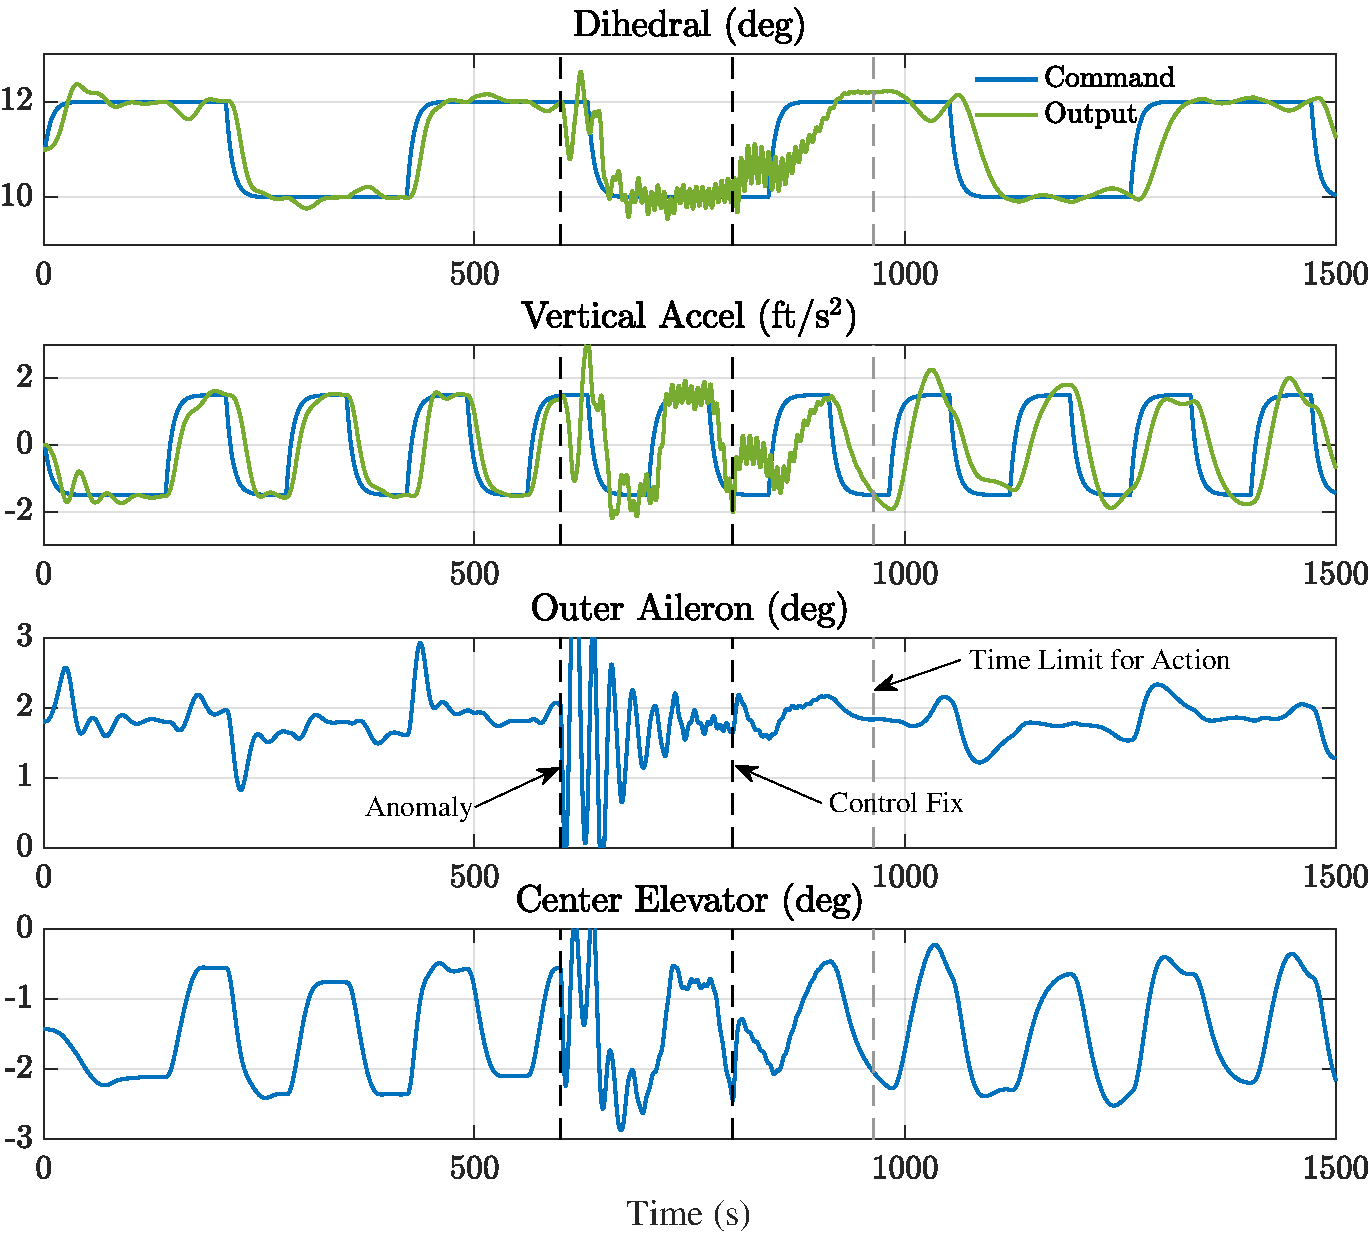
\includegraphics[width=\columnwidth]{ar3.pdf}
	\caption{AR-3 simulation: shared response to the dynamical anomaly results in recovery of vehicle performance}
	\label{fig:ar3-sim}
\end{figure}

\begin{figure}[htbp]
	\centering
	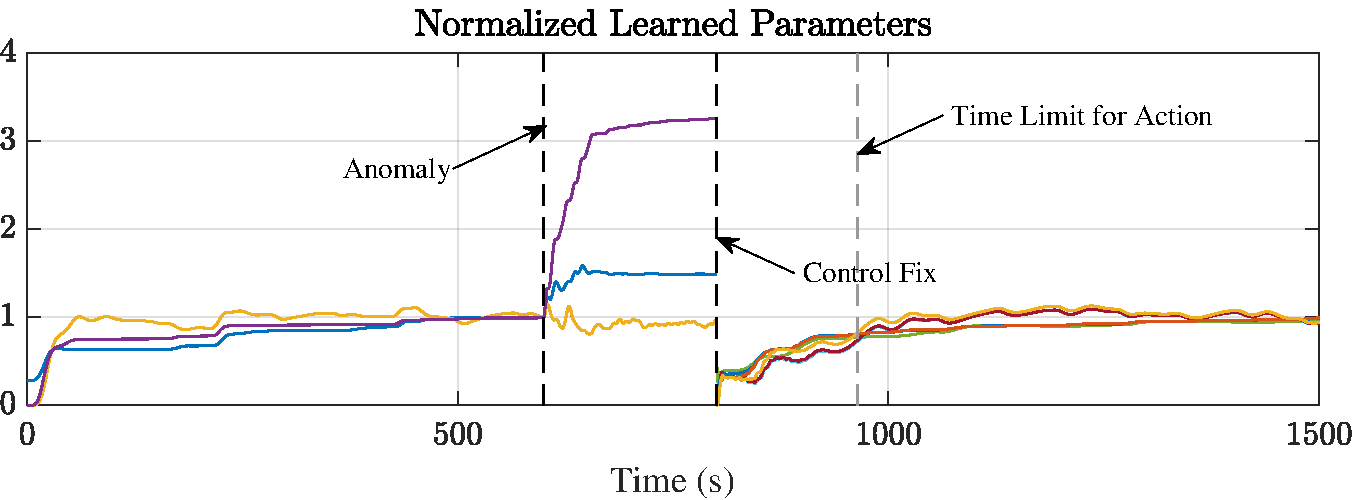
\includegraphics[width=\columnwidth]{ar3-params.pdf}
	\caption{AR-3 simulation: the change in control model at $t = 800 s$ stops the divergence of adaptive parameters}
	\label{fig:ar3-params}
\end{figure}

\begin{figure}[htbp]
	\centering
	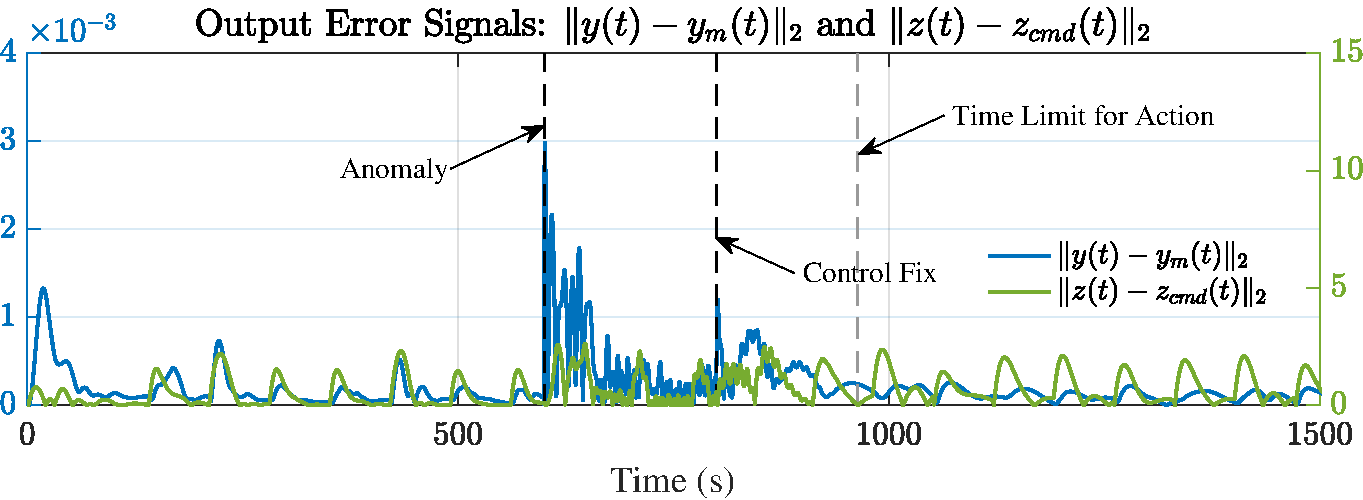
\includegraphics[width=\columnwidth]{ar3-err.pdf}
	\caption{AR-3 simulation: the change in control model at $t = 800 s$ stops the error growth seen after the anomaly}
	\label{fig:ar3-err}
\end{figure}

% Summary
\chapter{Concluding Remarks} \label{ch:conclusion}

This thesis developed a shared control architecture which synthesizes the actions of adaptive autopilots and human operators of aerial vehicles. Humans faced with the control of plants having unfamiliar dynamics attempt to adapt their control strategies, but their performance deteriorates while the risk of loss of control increases. Adaptive control algorithms can automate low-level control tasks, enabling stable and consistent closed-loop dynamic behavior when the parameters of open-loop plant dynamics are uncertain. The idea of this shared control architecture is to allow human operators to focus on higher-level perception and decision-making tasks where their cognitive capabilities can be leveraged, while using adaptive autopilots for command tracking and regulation tasks. The autonomous control algorithms presented in this thesis build on two recent advances in adaptive control theory, namely the use of closed-loop reference models for improved transient performance, and computationally efficient control designs for output-feedback systems having relative degree two or greater. 

In Chapter \ref{ch:siso_shared_ctrl} a shared control architecture between on-board human pilots and adaptive controllers with full state information was presented. In Chapter \ref{ch:mimo_shared_ctrl} the shared control architecture was developed for remote human operators and adaptive controllers having just partial state information available for feedback control. In these two settings, the human operator collaborates with the autopilot in the detection and diagnosis of the anomaly and relegates corrective actions to an adaptive flight control system. The targeted role of the human operator is motivated by the limitations that come with manual control of unfamiliar dynamical systems, as well as the cognitive and perceptive capabilities unique to human operators. Under our shared control framework, the human operator and adaptive autopilot designs form a shared response to dynamical anomalies. 

The shared controllers defined in Chapters \ref{ch:siso_shared_ctrl} and \ref{ch:mimo_shared_ctrl} are applied to several scenarios relevant to flight control through numerical simulations. The shared controller with on-board human pilots is demonstrated in the context of the roll dynamics of an aircraft, in the face of two different kinds of anomalies. In both cases, the pilot's task is to perceive if there is a change in the order of the vehicle dynamics, and convey this change to the adaptive autopilot. The resulting shared control action was shown to lead to satisfactory performance through detailed simulation studies. The shared control architecture using remote human operators is demonstrated in simulations of the longitudinal dynamics of an unmanned high altitude, long endurance aircraft. It is shown how an anomaly response using the shared controller is able to avert structural failure following an anomaly which abruptly changes actuator dynamics, and restore nominal performance.

There are several directions in which this work can be extended. One area to explore is in the development of anomaly detection and diagnosis tools to aid the human operator, based on models of how humans perceive and diagnose anomalies. Demonstrating this work on hardware platforms with a human in/on the loop is another area for future work which would provide valuable insights and help to bring this work to a higher level of maturity. In summary, designing control architectures which are able to leverage the benefits of both humans and model-based algorithmic controllers may allow for both safer and more performant systems compared to what is achievable using humans or autonomous controllers alone, and this thesis has demonstrated one of many possible realizations of such a control design philosophy.

\appendix
\chapter{Tables}

\begin{table}
\caption{Armadillos}
\label{arm:table}
\begin{center}
\begin{tabular}{||l|l||}\hline
Armadillos & are \\\hline
our	   & friends \\\hline
\end{tabular}
\end{center}
\end{table}

\clearpage
\newpage

%% This defines the bibliography file (main.bib) and the bibliography style.
%% If you want to create a bibliography file by hand, change the contents of
%% this file to a `thebibliography' environment.  For more information 
%% see section 4.3 of the LaTeX manual.
\begin{singlespace}
\bibliography{thomsen-thesis.bib}
\bibliographystyle{plain}
\end{singlespace}

\end{document}

